\documentclass{article}

% PACKAGES --------------------------------------------

% For layouts

\usepackage[english]{babel}
\usepackage[letterpaper,top=2cm,bottom=2cm,left=3cm,right=3cm,marginparwidth=1.75cm]{geometry}
\usepackage[skip=10pt plus1pt, indent=0pt]{parskip}
\usepackage{float}
% \usepackage[page]{appendix}


% For mathematical symbols
\usepackage{amsmath, amsfonts, amsthm, amssymb, gensymb, mathtools}


% For images, diagrams, boxed text and tables
\usepackage[usenames,dvipsnames, x11names, rgb]{xcolor}
\usepackage{graphicx}
\usepackage[]{mdframed}  % For boxed text
\usepackage{easytable}
\usepackage{tikz, pgfplots}
\pgfplotsset{compat=1.18}
% \usepackage{tikz-3dplot}
\usetikzlibrary{arrows.meta}
% \usetikzlibrary{calc}
% \usetikzlibrary{decorations.pathreplacing,calligraphy}  % Braces


% For links
\PassOptionsToPackage{hyphens}{url}\usepackage[hidelinks]{hyperref}


% For enumeration options
\usepackage{enumerate}


% For inference rules
\usepackage{proof}


% For resizing maths symbols
\usepackage{relsize}

% For code
\usepackage{listings}
\lstset{
  basicstyle=\ttfamily,
  columns=fullflexible,
  mathescape
}


% Font

% \usepackage{mathptmx}  % Times New Roman
% \usepackage{bookman}  % Bookman
% \usepackage{fourier}  % Fourier
% \usepackage{tgpagella}  % TeX Gyre Pagella


% -----------------------------------------------------

% Custom commands, environments, operators and other settings

\newcommand{\abs}[1]{|#1|}

\counterwithin*{equation}{section}

\newtheorem*{theorem}{Theorem}
% \newtheorem{corollary}{Corollary}[theorem]
\newtheorem*{lemma}{Lemma}

\DeclareMathOperator{\Rk}{Rk}


% -----------------------------------------------------

% Color scheme for TikZ diagrams:
% MidnightBlue
% OliveGreen
% BrickRed
% BurntOrange
% Fuchsia

% -----------------------------------------------------

\title{Notes for Logic (COMP0009)}
\author{Raphael Li}
\date{Sep 2025}


\begin{document}
\maketitle

\vspace{1em}
\hrule
\vspace{1em}


\tableofcontents

\newpage
\section{Revision: The syntax and semantics of propositional and first-order logic}

Formally, a \emph{logic} consists of three components:

\begin{table}[H]
    \centering
    \begin{tabular}{|c|c|}
        \hline
        \textbf{Component} & \textbf{Describes...}\\
        \hline
        Syntax & The language and grammar for writing formulas\\
        \hline
        Semantics & How formulas are interpreted\\
        \hline
        Inference system (or proof system) & A syntactic device for proving true statements\\
        \hline
    \end{tabular}

    \caption{The three key components of a logic.}
    \label{tab:Ch01-components-of-a-logic}
\end{table}

This module concerns algorithms that automatically parse and determine the validity of a formula.


\subsection{Propositional logic}

\subsubsection{Syntax}

Formulas are constructed by applying negation, conjunction and disjunction to propositions. 
%
\begin{align*}
    \text{proposition} &\coloneq p \;\vert\; q \;\vert\; r \;\vert\; \cdots\\
    \text{formula} &\coloneq \text{proposition} \;\vert\; \neg \text{formula} \;\vert\; (\text{formula} \circ \text{formula})  \tag{where \(\circ\) is \(\land\), \(\lor\) or \(\rightarrow\)}
\end{align*}
%
A proposition or its negation is called a \emph{literal}\footnote{For example, \(p\) and \(\neg p\) are both literals, but \(\neg\neg q\) is not.}.

For any formula that isn't a proposition, the \emph{main connective} is the one with the largest scope. In other words, it is not in the scope of any other connective.
%
\[((p \land q) \;{\color{BrickRed} \lor}\; \neg (q \rightarrow r))\]
%
This is the connective with which evaluation begins. This is especially important when building parsers for algorithmically evaluating formulas.

Note that parsers working according to the above definition will recognise \((p \land q)\), but not \(p \land q\), as a formula. Regardless, throughout this document we will use a looser definition where brackets may be ommitted in unambiguous cases.


\subsubsection{Semantics}

A valuation is a function \(v\) that maps each proposition to a truth value in \(\{\top, \bot\}\).
    
\begin{figure}[H]
    \centering
    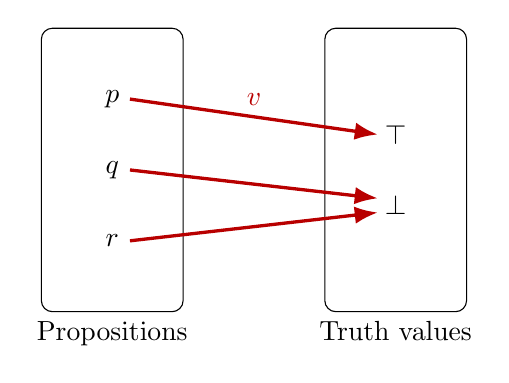
\begin{tikzpicture}[scale=0.9]
        \draw[rounded corners] (-3, 0) rectangle (-1, -4) {};
        \draw[rounded corners] (1, 0) rectangle (3, -4) {};

        \node[align=center, anchor=center] at (-2, -1) {\(p\)};
        \node[align=center, anchor=center] at (-2, -2) {\(q\)};
        \node[align=center, anchor=center] at (-2, -3) {\(r\)};

        \node[align=center, anchor=center] at (2, -1.5) {\(\top\)};
        \node[align=center, anchor=center] at (2, -2.5) {\(\bot\)};

        \draw[-Latex, very thick, BrickRed] (-1.75, -1) -- (1.75, -1.5) node[pos=0.5, anchor=south] {\(v\)};

        \draw[-Latex, very thick, BrickRed] (-1.75, -2) -- (1.75, -2.4);

        \draw[-Latex, very thick, BrickRed] (-1.75, -3) -- (1.75, -2.6);

        \node[anchor=north] at (-2, -4) {Propositions};

        \node[anchor=north] at (2, -4) {Truth values};
        
    \end{tikzpicture}
    \caption{A valuation maps propositions to truth values.}
    \label{fig:Ch01-valuation}
\end{figure}

A valuation \(v\) can be extended to a unique \emph{truth function} defined on all possible formulas. A truth function \(v'\) must satisfy
%
\begin{align*}
    v'(\neg \phi) = \top &\iff v'(\phi) = \bot\\
    v'(\phi \lor \psi) = \top &\iff v'(\phi) = \top \text{ or } v'(\psi) = \top\\
    v'(\phi \land \psi) = \top &\iff v'(\phi) = \top \text{ and } v'(\psi) = \top\\
    v'(\phi \rightarrow \psi) = \top &\iff v'(\phi) = \bot \text{ or } v'(\psi) = \top\\
    v'(\phi \leftrightarrow \psi) = \top &\iff v'(\phi) = v'(\psi)
\end{align*}
%
for all formulas \(\phi\) and \(\psi\). From now on we use \(v\) to denote the more general truth function.

The result of applying a valuation \(v\) to a formula \(\phi\) depends only on the propositional letters that occur in \(\phi\). 

A formula \(\phi\) is \emph{valid} if \(v(\phi) = \top\) for all valuations \(v\), which we denote as \(\models \phi\). A formula \(\phi\) is \emph{satisfiable} if \(v(\phi) = \top\) for at least one valuation \(v\). All valid formulas are satisfiable, but \emph{not} vice versa.

Two formulas \(\phi\) and \(\psi\) are \emph{logically equivalent}, written as \(\phi \equiv \psi\), if and only if for every valuation \(v\) we have \(v(\phi) = v(\psi)\).



\subsubsection{Truth tables}

Consider the propositional formula \(((p \lor \neg q) \land \neg (q \land r))\). We can check its validity and satisfiability by constructing its truth table.

\begin{table}[H]
    \centering
    \begin{tabular}{|c|c|c||c|c||c|}
        \hline
        \(p\) & \(q\) & \(r\) & \((p \lor \neg q)\) & \(\neg (q \land r)\) & \(((p \lor \neg q) \land \neg (q \land r))\)\\
        \hline
        0 & 0 & 0 & 1 & 1 & 1 \\
        \hline
        0 & 0 & 1 & 1 & 1 & 1 \\
        \hline
        0 & 1 & 0 & 0 & 1 & 0 \\
        \hline
        0 & 1 & 1 & 0 & 0 & 0\\
        \hline
        1 & 0 & 0 & 1 & 1 & 1 \\
        \hline
        1 & 0 & 1 & 1 & 1 & 1 \\
        \hline
        1 & 1 & 0 & 1 & 1 & 1 \\
        \hline
        1 & 1 & 1 & 1 & 0 & 0 \\
        \hline
    \end{tabular}

    \caption{The truth table for the formula \(((p \lor \neg q) \land \neg (q \land r))\).}
    \label{tab:Ch01-truth-table}
\end{table}

In this case, the formula is satisfiable but not valid.



\subsubsection{Parse trees}

A parser interprets the semantics of a formula by breaking down its symbols into a \emph{parse tree}, which shows the syntactic relation between symbols. For example, the formula \(((p \lor \neg q) \land \neg (q \land r))\) can be broken down into the following parse tree.

\begin{figure}[H]
    \centering
    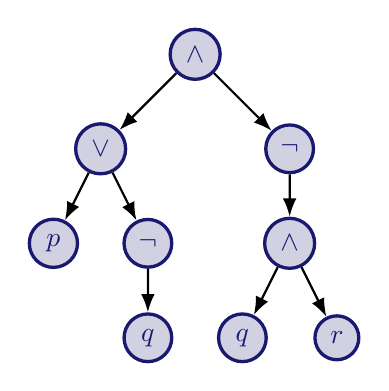
\begin{tikzpicture}[scale=0.6]
        \node (main-and) at (0,0)[circle, draw=MidnightBlue, very thick, MidnightBlue, fill=MidnightBlue!20] {\(\land\)};
        \node (or) at (-2,-2)[circle, draw=MidnightBlue, very thick, MidnightBlue, fill=MidnightBlue!20] {\(\lor\)};
        \node (right-neg) at (2,-2)[circle, draw=MidnightBlue, very thick, MidnightBlue, fill=MidnightBlue!20] {\(\neg\)};
        \node (p) at (-3,-4)[circle, draw=MidnightBlue, very thick, MidnightBlue, fill=MidnightBlue!20] {\(p\)};
        \node (left-neg) at (-1,-4)[circle, draw=MidnightBlue, very thick, MidnightBlue, fill=MidnightBlue!20] {\(\neg\)};
        \node (and) at (2,-4)[circle, draw=MidnightBlue, very thick, MidnightBlue, fill=MidnightBlue!20] {\(\land\)};
        \node (left-q) at (-1,-6)[circle, draw=MidnightBlue, very thick, MidnightBlue, fill=MidnightBlue!20] {\(q\)};
        \node (right-q) at (1,-6)[circle, draw=MidnightBlue, very thick, MidnightBlue, fill=MidnightBlue!20] {\(q\)};
        \node (r) at (3,-6)[circle, draw=MidnightBlue, very thick, MidnightBlue, fill=MidnightBlue!20] {\(r\)};

        \draw[-Latex, thick] (main-and) -- (or);
        \draw[-Latex, thick] (main-and) -- (right-neg);
        \draw[-Latex, thick] (or) -- (p);
        \draw[-Latex, thick] (or) -- (left-neg);
        \draw[-Latex, thick] (right-neg) -- (and);
        \draw[-Latex, thick] (left-neg) -- (left-q);
        \draw[-Latex, thick] (and) -- (right-q);
        \draw[-Latex, thick] (and) -- (r);
    \end{tikzpicture}
    \caption{The parse tree for the formula \(((p \lor \neg q) \land \neg (q \land r))\).}
    \label{fig:Ch01-parse-tree}
\end{figure}



\subsubsection{Disjunctive normal form (DNF)}

A formula is said to be in \emph{disjunctive normal form} (DNF) if it is a disjunction of one or more conjunctions of one or more literals.
%
\begin{align*}
    \text{proposition} &\coloneq p \;\vert\; q \;\vert\; r \;\vert\; \cdots\\
    \text{literal} &\coloneq \text{proposition} \;\vert\; \neg\text{proposition}\\
    \text{conjunctiveClause} &\coloneq \text{literal} \;\vert\; \text{literal } \land \text{ conjunctiveClause}\\
    \text{DNF} &\coloneq \text{conjunctiveClause} \;\vert\; \text{conjunctiveClause } \lor \text{ DNF}
\end{align*}
%
Below is an example of a formula in DNF.
%
\[
    {\color{BrickRed}\underbrace{(p \land \neg q \land \neg r)}_{\substack{\text{conjunctive}\\\text{clause}}}}
    \lor
    {\color{BrickRed}\underbrace{(\neg p \land \neg q \land r)}_{\substack{\text{conjunctive}\\\text{clause}}}}
    \lor
    {\color{BrickRed}\underbrace{(q \land \neg r)}_{\substack{\text{conjunctive}\\\text{clause}}}}
\]

Any propositional formula has a DNF equivalent. For instance, the formula \((p \lor \neg q) \land \neg (q \land r)\) can be rewritten as follows.
%
\begin{align*}
    & (p \lor \neg q) \land \neg (q \land r)\\
    \iff & (p \lor \neg q) \land (\neg q \lor \neg r) \tag{De Morgan's law, to remove outer negation}\\
    \iff & {\color{BrickRed}((p \lor \neg q) \land \neg q)} \lor {\color{MidnightBlue}((p \lor \neg q) \land \neg r)} \tag{distributing conjunctions over disjunctions}\\
    \iff & {\color{BrickRed}(p \land \neg q) \lor (\neg q \land \neg q)} \lor {\color{MidnightBlue}(p \land \neg r) \lor (\neg q \land \neg r)} \tag{distributing conjunctions over disjunctions}\\
    \iff & {\color{BrickRed}(p \land \neg q) \lor \neg q} \lor {\color{MidnightBlue}(p \land \neg r) \lor (\neg q \land \neg r)}
\end{align*}

Alternatively, this can also be achieved by referring to the truth table. From Table \ref{tab:Ch01-truth-table}, we see that the formula can be written in DNF as
%
\[(\neg p \land \neg q \land \neg r) \lor (\neg p \land \neg q \land r) \lor (p \land \neg q \land \neg r)  \lor (p \land \neg q \land r)  \lor (p \land q \land \neg r)\text{.}\]



\subsubsection{Conjunctive normal form (CNF)}

A formula is said to be \emph{conjunctive normal form} (CNF) if it is a conjunction of one or more disjunctions of one or more literals.
%
\begin{align*}
    \text{disjunctiveClause} &\coloneq \text{literal} \;\vert\; \text{literal } \lor \text{ disjunctiveClause}\\
    \text{CNF} &\coloneq \text{disjunctiveClause} \;\vert\; \text{disjunctiveClause } \land \text{ CNF}
\end{align*}
%
Below is a formula in CNF.
%
\[
    {\color{BrickRed}\underbrace{(p \lor \neg q \lor \neg r)}_{\substack{\text{conjunctive}\\\text{clause}}}}
    \land
    {\color{BrickRed}\underbrace{(\neg p \lor q \lor r)}_{\substack{\text{conjunctive}\\\text{clause}}}}
\]

To find the CNF equivalent of a formula \(\phi\), we first express its negation \(\neg\phi\) in DNF. Then, we negate it again to get \(\neg\neg\phi\). Using De Morgan's law, the resultant formula will be in CNF.

For example, let \(\phi\) be the formula \((p \lor \neg q) \land \neg (q \land r)\). To rewrite it in CNF, we start by constructing the truth table of its negation \(\neg\phi\). This allows us to express \(\neg\phi\) in DNF.

\begin{table}[H]
    \centering
    \begin{tabular}{|c|c|c||c|c|}
        \hline
        \(p\) & \(q\) & \(r\) & \(((p \lor \neg q) \land \neg (q \land r))\) & Negation of \(((p \lor \neg q) \land \neg (q \land r))\)\\
        \hline
        0 & 0 & 0 & 1 & 0 \\
        \hline
        0 & 0 & 1 & 1 & 0 \\
        \hline
        0 & 1 & 0 & 0 & 1 \\
        \hline
        0 & 1 & 1 & 0 & 1 \\
        \hline
        1 & 0 & 0 & 1 & 0 \\
        \hline
        1 & 0 & 1 & 1 & 0 \\
        \hline
        1 & 1 & 0 & 1 & 0 \\
        \hline
        1 & 1 & 1 & 0 & 1 \\
        \hline
    \end{tabular}

    \caption{The truth table for the negation of \(((p \lor \neg q) \land \neg (q \land r))\). This is obtained by flipping the results of Table \ref{tab:Ch01-truth-table}.}
    \label{tab:Ch01-truth-table-of-negation}
\end{table}

Hence we have
%
\begin{align*}
    \neg\phi &= (\neg p \land q) \lor (p \land q \land r) \tag{DNF of \(\neg\phi\)}\\
    \neg\neg\phi &= \neg((\neg p \land q) \lor (p \land q \land r)) \tag{negating both sides}\\
    \phi &= (p \lor \neg q) \land (\neg p \lor \neg q \lor \neg r) \tag{double negation; De Morgan's laws}
\end{align*}
%
which gives us \(\phi\) in CNF.



\subsection{First-order logic}

\subsubsection{Syntax}

A first-order language \(L(C, F, P)\) is determined by a set \(C\) of constant symbols, a set \(F\) of function symbols and a non-empty set \(P\) of predicate symbols. Each function symbol and predicate symbol has an associated \emph{arity} \(n \in \mathbb{N}\). We write \(f^n\) and \(p^n\) to represent an \(n\)-ary function symbol and an \(n\)-ary predicate symbol respectively. Moreover, let \(V\) be a countably infinite set of variable symbols.
%
\begin{align*}
    \text{term} &\coloneq c \;\vert\; v \;\vert\; f^n (\text{term}_0, \text{term}_1, \cdots, \text{term}_{n-1}) \tag{where \(c \in C\), \(v \in V\) and \(f^n \in F\)}\\
    \text{atom} &\coloneq p^n (\text{term}_0, \text{term}_1, \cdots, \text{term}_{n-1}) \tag{where \(p^n \in P\)}\\
    \text{formula} &\coloneq \text{atom} \;\vert\; \neg \text{formula} \;\vert\; (\text{formula}_0 \lor \text{formula}_1) \;\vert\; \exists v\; \text{formula}  \tag{where \(v \in V\)}
\end{align*}
%
This definition is functionally complete. Formulas involving universal quantifiers, implications and equivalence symbols can always be rewritten using only symbols defined above.

A \emph{closed term} is a term with no variable symbols. A \emph{sentence} is a formula with no free variables.



\subsubsection{Semantics}

For a first-order language \(L(C, F, P)\), we may construct a corresponding first-order structure\footnote{Also known as an \(L\)-structure.} \(S = (D, I)\) where \(I = (I_c, I_f, I_p)\).
%
{\large
    \[
        S = (
            {\color{BrickRed}
                \underbrace{D}_{\substack{
                    \text{non-empty}\\
                    \text{domain}
                }}
            }
            ,
            {\color{MidnightBlue}
                \overbrace{(
                    I_c,
                    I_f,
                    I_p
                )}^{\text{interpretation } I}
            }
        )
    \]
}
%
Here,
\begin{itemize}
    \item \(I_c\) maps each constant symbol in \(C\) to an element of \(D\).
    \item \(I_f\) maps each \(n\)-ary function symbol in \(F\) to an \(n\)-ary function over \(D\).
    \item \(I_p\) maps each \(n\)-ary predicate symbol \(p \in P\) to an \(n\)-ary relation over \(D\) (i.e. a subset of \(D^n\)).
    \item We may occasionally use \(I\) to denote a general interpretation function where
    %
    \begin{align*}
        I(c) &= I_c (c) \tag{for all \(c \in C\)}\\
        I(f) &= I_f (f) \tag{for all \(f \in F\)}\\
        I(p) &= I_p (p) \tag{for all \(p \in P\)}
    \end{align*}
\end{itemize}

If \(P\) includes the equality symbol \(=\), then it is always interpreted as the binary relation of true equality.
%
\[I_p (=) = \{(d, d) : d \in D\}\]

Given a structure \(S = (D, I)\), a variable assignment \(A\) is a map from \(V\) to \(D\). For any variable \(v \in V\), two variable assignments \(A\) and \(A^{*}\) are said to be \(v\)-equivalent if \(A(x) = A^{*}(x)\) for all \(x \in V \setminus \{v\}\). In other words, two variable assignments are said to be \(v\)-equivalent if they are completely identical except possibly for the element in \(D\) assigned to \(v\). This is written as \(A \equiv_v A^{*}\).

Given a structure \(S\) and a variable assignment \(A\), we may interpret any term as follows.
%
\begin{align*}
    c^{S, A} &= I_c (c)\\
    v^{S, A} &= A(v)\\
    f^n (t_0, t_1, \cdots, t_{n-1})^{S, A} &= {\color{MidnightBlue} \underbrace{(I_f (f^n))}_{\substack{\text{interpreted}\\\text{function}}}} (t_0^{S, A}, t_1^{S, A}, \cdots, t_{n-1}^{S, A})
\end{align*}

Formulas are evaluated as follows.
%
\begin{align*}
    S \models_A p^n (t_0, t_1, \cdots, t_{n-1}) &\iff (t_0^{S, A}, t_1^{S, A}, \cdots, t_{n-1}^{S, A}) \in I_p (p^n)\\
    S \models_A \neg \text{formula} &\iff S \not\models_A \text{formula}\\
    S \models_A (\text{formula}_0 \lor \text{formula}_1) &\iff S \models_A \text{formula}_0 \text{ or } S \models_A \text{formula}_1\\
    % S \models_A (\text{formula}_0 \land \text{formula}_1) &\iff S \models_A \text{formula}_0 \text{ and } S \models_A \text{formula}_1\\
    % S \models_A (\text{formula}_0 \rightarrow \text{formula}_1) &\iff S \not\models_A \text{formula}_0 \text{ or } S \models_A \text{formula}_1\\
    S \models_A \exists v\; \text{formula} &\iff S \models_{A[x \mapsto d]} \text{formula for some } d \in D
\end{align*}

Given a structure \(S\) and a formula \(\phi\), we say that
%
\begin{itemize}
    \item \(\phi\) is ``valid in \(S\)'' if \(S \models_A \phi\) for every variable assignment \(A\). This is written as \(S \models \phi\).
    \item \(\phi\) is ``satisfiable in \(S\)'' if \(S \models_A \phi\) for some variable assignment \(A\).
    \item \(\phi\) is ``valid'' if \(\phi\) is valid in all possible structures. This is written as \(\models \phi\).
    \item \(\phi\) is ``satisfiable'' if there exists some structure in which \(\phi\) is satisfiable.
\end{itemize}
%
A formula \(\phi\) is valid if and only if \(\neg \phi\) is not satisfiable.
%
\begin{quote}
    \textbf{Proof.} Let \(\neg\phi\) be a formula that is not satisfiable. Hence we have
    %
    \begin{align*}
        \neg \exists S\; \exists A\;\;\; S \models_A \neg\phi &\iff \neg \exists S\; \exists A\;\;\; S \not\models_A \phi\\
        &\iff \forall S\; \neg \exists A\;\;\; S \not\models_A \phi\\
        &\iff \forall S\; \forall A\;\;\;  \neg S \not\models_A \phi\\
        &\iff \forall S\; \forall A\;\;\; S \models_A \phi
    \end{align*}
    %
    which means \(S\) is valid.
\end{quote}

If \(\phi\) is a sentence, then \(\phi\) is valid in \(S\) if and only if it is also satisfiable in \(S\).



\subsubsection{Example: Arithmetic in the set of natural numbers}

Consider the first-order language \(L(C, F, P)\) defined as follows. Also assume a countably infinite set \(V\) of variable symbols.
%
\begin{align*}
    C &= 1, 2, 3, \cdots \tag{constant symbols}\\
    F &= \{+, \times\} \tag{function symbols, both binary}\\
    P &= \{=, <\} \tag{predicate symbols, both binary}\\
    V &= \{x, y, z, \cdots\} \tag{variable symbols}
\end{align*}
%
A term is a string of symbols that represents a ``thing'' or an ``object'' --- this can be a constant, a variable, or a function output.
%
\begin{itemize}
    \item \(x\)
    \item \(1 + 3\)
    \item \(2 \times x + 1\)
\end{itemize}
%
Of the terms shown above, only the second one is a closed terms because it has no variable symbols.

An atom is a string of symbols that represents the output of a predicate, which is a truth value.
%
\begin{itemize}
    \item \(1 = 2\)
    \item \(y < 3\)
    \item \(x + 1 < 2 \times z + 3\)
\end{itemize}
%
Finally, a formula is constructed by applying negations, disjunctions, and existential quantifiers to atoms.
%
\begin{itemize}
    \item \(1 = 2 \;\land\; y < 3\)
    \item \(\neg \exists z\;\; x + 1 < 2 \times z + 3\)
\end{itemize}
%
The latter example is a sentence because all of its variable symbols are bounded.

For this particular first-order language, we may use the structure of ordinary arithmetic\footnote{There is also a similar structure \(R = (\mathbb{R}, I)\) where the domain is the set of real numbers.}, defined as \(N = \{\mathbb{N}, \{I_c, I_f, I_p\}\}\) where
%
\begin{itemize}
    \item \(I_c\) is a function that maps numerical symbols to the corresponding natural number.
    %
    \begin{align*}
        I_c (1) &= 1\\
        I_c (2) &= 2\\
        I_c (3) &= 3\\
        &\;\;\vdots
    \end{align*}

    \item \(I_f\) maps \(+\) and \(\times\) to the addition and multiplication operations in arithmetic respectively.
    
    \item \(I_p\) maps \(=\) and \(<\) to the following relations.
    %
    \begin{align*}
        I_p (=) &= \{(n, n) : n \in \mathbb{N}\}\\
        I_p (<) &= \{(m, n) \in \mathbb{N}^2 : m < n\}
    \end{align*}
\end{itemize}



\subsubsection{First-order structures and directed graphs}

Consider a first-order language with only one binary predicate symbol \(p\).
%
\[L(C, F, {\color{BrickRed} \{p\}})\]
%
Any first-order structure \(S = \{D, \{I_c, I_f, I_p\}\}\) for this language can be represented as a directed graph, where each vertex is an element of \(D\) and each directed edge represents an element of the relation \(I_p (p)\).

\begin{figure}[H]
    \centering
    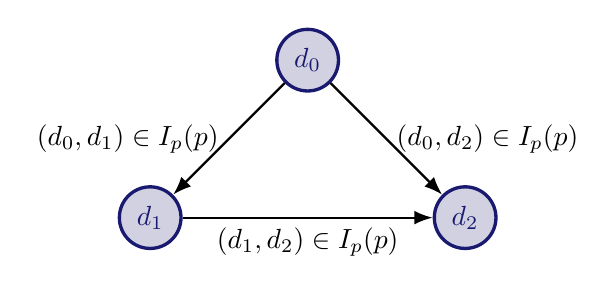
\begin{tikzpicture}
        \node (d0) at (0,0)[circle, draw=MidnightBlue, very thick, MidnightBlue, fill=MidnightBlue!20] {\(d_0\)};
        \node (d1) at (-2,-2)[circle, draw=MidnightBlue, very thick, MidnightBlue, fill=MidnightBlue!20] {\(d_1\)};
        \node (d2) at (2,-2)[circle, draw=MidnightBlue, very thick, MidnightBlue, fill=MidnightBlue!20] {\(d_2\)};

        \draw[-Latex, thick] (d0) -- (d1) node[pos=0.5, left]{\((d_0, d_1) \in I_p (p)\)};

        \draw[-Latex, thick] (d0) -- (d2) node[pos=0.5, right]{\((d_0, d_2) \in I_p (p)\)};

        \draw[-Latex, thick] (d1) -- (d2) node[pos=0.5, below]{\((d_1, d_2) \in I_p (p)\)};
        
    \end{tikzpicture}
    \caption{The first-order structure \(S\) can be visualised as a directed graph.}
    \label{fig:Ch01-first-order-structure-as-directed-graph}
\end{figure}

\newpage
\section{Axiomatic Proofs for Propositional Logic}

A \emph{proof system} is a system for determining the validity of formulas.

An obvious system would be to construct a truth table and check that all rows give a true result. However, this naive approach has an exponential time complexity\footnote{Using this system, checking the validity of a formula with \(n\) proposition symbols requires \(2^n\) computations.}, meaning that it will become increasingly impractical as more and more propositions are introduced. To alleviate this issue, we will introduce a different approach below.



\subsection{Axiomatic proof system}

Firstly, we limit our propositional language to only use the connectives \(\neg\) and \(\rightarrow\). Double negations are prohibited.

Moreover, we will note some \emph{axioms} that are known to be valid, and then try to derive other valid formulas from the axioms. Below we list three different \emph{schemas}, from which axioms may be obtained by substituting any formulas in place of \(p\), \(q\) and \(r\).
%
\begin{enumerate}[I.]
    \item \(p \rightarrow (q \rightarrow p)\)
    \item \((p \rightarrow (q \rightarrow r)) \rightarrow ((p \rightarrow q) \rightarrow (p \rightarrow r))\)
    \item \((\neg p \rightarrow \neg q) \rightarrow (q \rightarrow p)\)
\end{enumerate}

Axioms on their own are insufficient in establishing a proof system. We also need \emph{inference rules}, which stipulate how conclusions can be derived from premises. One of the main inference rules is \emph{modus ponens}, which states that if you have proved both the formula \(\phi\) and the implication \((\phi\rightarrow\psi)\), then you may deduce the conclusion \(\psi\).
%
\[
    \infer{\psi}{
        \phi
        &
        (\phi\rightarrow\psi)
    }
    %
    \tag{modus ponens}
\]

In this system, a \emph{proof} is a sequence of formulas
%
\[\phi_0,\; \phi_1,\; \phi_2,\; \cdots \phi_n\]
%
such that for each \(i \leq n\), the formula \(\phi_i\) is either
%
\begin{itemize}
    \item an axiom; or
    \item obtained from two previous formulas \(\phi_j\) and \(\phi_k\) in the sequence via modus ponens (for some \(j, k < i\)).
\end{itemize}
%
If such a proof exists, then the final formula \(\phi_n\) is called a \emph{theorem} and we may write \(\vdash \phi_n\).

\begin{figure}[H]
    \centering
    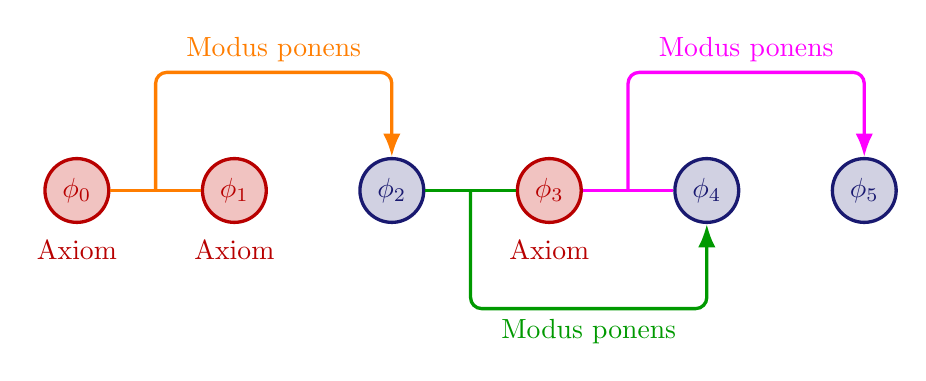
\begin{tikzpicture}
        \foreach \i in {0,1,3} {
            \node (\i) at (2*\i, 0)[circle, draw=BrickRed, very thick, BrickRed, fill=BrickRed!20] {\(\phi_\i\)};

            \draw node[yshift=-0.75cm, BrickRed] at (2*\i, 0) {Axiom};
        }

        \foreach \i in {2,4,5} {
            \node (\i) at (2*\i, 0)[circle, draw=MidnightBlue, very thick, MidnightBlue, fill=MidnightBlue!20] {\(\phi_\i\)};
        }

        \draw[BurntOrange, very thick] (0) -- (1);
        \draw[BurntOrange, very thick, -Latex, rounded corners] (1, 0) -- (1, 1.5) -- (4,1.5) node[pos=0.5, above]{Modus ponens} -- (2);
        
        \draw[OliveGreen, very thick] (2) -- (3);
        \draw[OliveGreen, very thick, -Latex, rounded corners] (5, 0) -- (5, -1.5) -- (8,-1.5) node[pos=0.5, below]{Modus ponens} -- (4);
        
        \draw[Fuchsia, very thick] (3) -- (4);
        \draw[Fuchsia, very thick, -Latex, rounded corners] (7, 0) -- (7, 1.5) -- (10,1.5) node[pos=0.5, above]{Modus ponens} -- (5);
    \end{tikzpicture}
    \caption{In a proof, every formula must be either an axiom, or derived from previous formulas via modus ponens.}
    \label{fig:Ch02-proof}
\end{figure}



\newpage
\section{Propositional tableau}

In view of the impracticality of Hilbert-style proof systems, we introduce below an easier and more implementable method for determining a formula's validity --- \emph{tableaus}.

Here is a brief overview of how a tableau works. Suppose we want to check the satisfiability of a formula \(\phi\). This formula will be placed at the root of a binary tree, called a tableau. We use a variety of expansion rules to grow the tree until it is complete. An \emph{open} tableau indicates that \(\phi\) is satisfiable, while a \emph{closed} tableau indicates that \(\phi\) is unsatisfiable.

To determine the validity of a formula, simply construct a tableau for \(\neg\phi\). If the resultant tableau is open, then \(\neg\phi\) is satisfiable, so \(\phi\) is invalid. On the contrary, if the resultant tableau is closed, then \(\neg\phi\) must be unsatisfiable, so \(\phi\) is valid.


\subsection{Constructing a tableau}

In a tableau, every node is marked with a formula. To build a tableau for a formula \(\phi\), begin by placing \(\phi\) at the root of a binary tree. Then, we repeat the following process:
%
\begin{enumerate}
    \item Select a formula in the tree that has not been selected before. The formula must not be a literal.
    \item Choose the expansion rule (see below) that applies to the selected formula.
    \item For each leaf node, add new children nodes in accordance to the chosen expansion rule.
    \item Place a tick beside the selected formula to make sure we don't expand it again.
\end{enumerate}

There are two types of expansion rules:
%
\begin{itemize}
    \item \(\alpha\)-rules, which create one new child per leaf node; and
    \item \(\beta\)-rules, which create two new children per leaf node.
\end{itemize}

Figures \ref{fig:Ch03-alpha-rules} and \ref{fig:Ch03-beta-rules} depict the \(\alpha\)- and \(\beta\) rules respectively. Nodes that are newly created by each rule are highlighted in blue.


\begin{figure}[H]
    \centering
    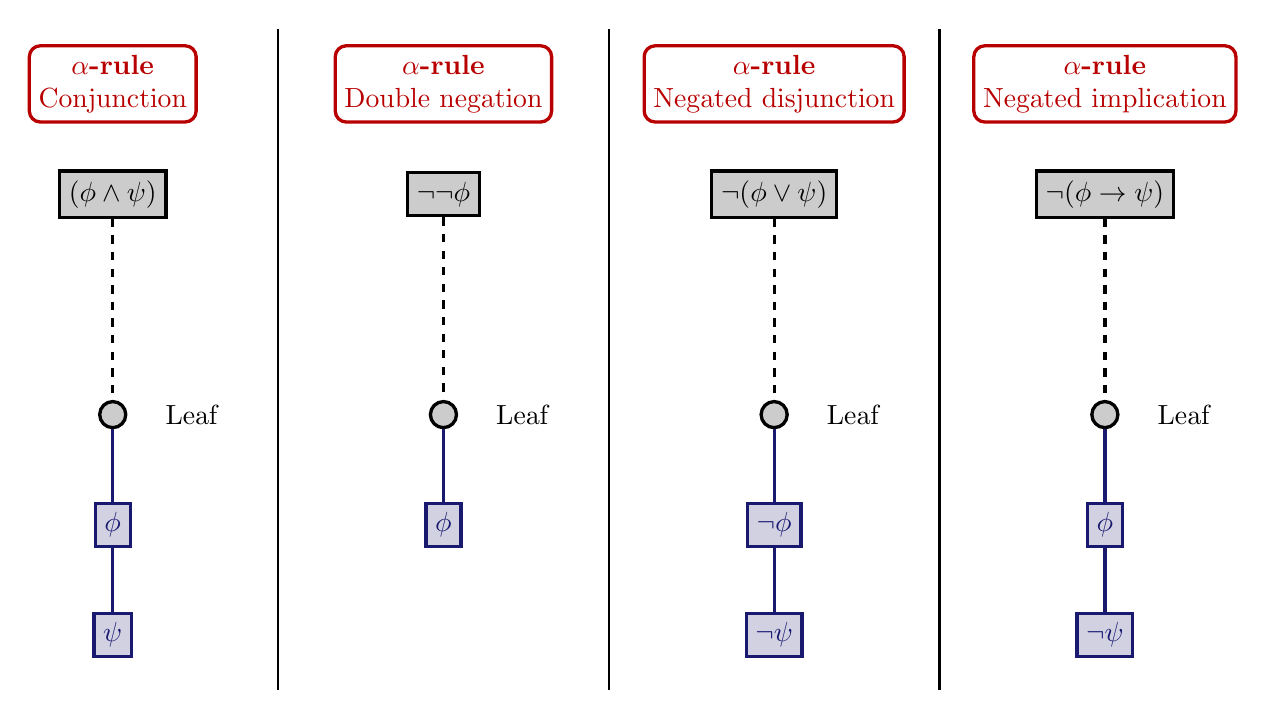
\begin{tikzpicture}[scale=1.4]
        \begin{scope}[shift={(0, 0)}]
            \node (root) at (0, 1)[draw=BrickRed, very thick, BrickRed, rounded corners, align=center] {\textbf{\(\alpha\)-rule} \\ Conjunction};

            \node (root) at (0, 0)[draw=black, very thick, fill=black!20] {\((\phi\land\psi)\)};

            \node (leaf) at (0, -2)[circle, draw=black, very thick, fill=black!20] {};

            \node [right of=leaf, black] {Leaf};

            \draw[dashed, very thick] (root) -- (leaf);

            \node (child1) at (0, -3)[draw=MidnightBlue, very thick, MidnightBlue, fill=MidnightBlue!20] {\(\phi\)};

            \node (child2) at (0, -4)[draw=MidnightBlue, very thick, MidnightBlue, fill=MidnightBlue!20] {\(\psi\)};

            \draw[very thick, MidnightBlue] (leaf) -- (child1) -- (child2);
        \end{scope}

        \begin{scope}[shift={(3, 0)}]
            \node (root) at (0, 1)[draw=BrickRed, very thick, BrickRed, rounded corners, align=center] {\textbf{\(\alpha\)-rule} \\ Double negation};

            \node (root) at (0, 0)[draw=black, very thick, fill=black!20] {\(\neg\neg\phi\)};

            \node (leaf) at (0, -2)[circle, draw=black, very thick, fill=black!20] {};

            \node [right of=leaf, black] {Leaf};

            \draw[dashed, very thick] (root) -- (leaf);

            \node (child1) at (0, -3)[draw=MidnightBlue, very thick, MidnightBlue, fill=MidnightBlue!20] {\(\phi\)};

            \draw[very thick, MidnightBlue] (leaf) -- (child1);
        \end{scope}

        \begin{scope}[shift={(6, 0)}]
            \node (root) at (0, 1)[draw=BrickRed, very thick, BrickRed, rounded corners, align=center] {\textbf{\(\alpha\)-rule} \\ Negated disjunction};

            \node (root) at (0, 0)[draw=black, very thick, fill=black!20] {\(\neg(\phi\lor\psi)\)};

            \node (leaf) at (0, -2)[circle, draw=black, very thick, fill=black!20] {};

            \node [right of=leaf, black] {Leaf};

            \draw[dashed, very thick] (root) -- (leaf);

            \node (child1) at (0, -3)[draw=MidnightBlue, very thick, MidnightBlue, fill=MidnightBlue!20] {\(\neg\phi\)};

            \node (child2) at (0, -4)[draw=MidnightBlue, very thick, MidnightBlue, fill=MidnightBlue!20] {\(\neg\psi\)};

            \draw[very thick, MidnightBlue] (leaf) -- (child1) -- (child2);
        \end{scope}

        \begin{scope}[shift={(9, 0)}]
            \node (root) at (0, 1)[draw=BrickRed, very thick, BrickRed, rounded corners, align=center] {\textbf{\(\alpha\)-rule} \\ Negated implication};

            \node (root) at (0, 0)[draw=black, very thick, fill=black!20] {\(\neg(\phi\rightarrow\psi)\)};

            \node (leaf) at (0, -2)[circle, draw=black, very thick, fill=black!20] {};

            \node [right of=leaf, black] {Leaf};

            \draw[dashed, very thick] (root) -- (leaf);

            \node (child1) at (0, -3)[draw=MidnightBlue, very thick, MidnightBlue, fill=MidnightBlue!20] {\(\phi\)};

            \node (child2) at (0, -4)[draw=MidnightBlue, very thick, MidnightBlue, fill=MidnightBlue!20] {\(\neg\psi\)};

            \draw[very thick, MidnightBlue] (leaf) -- (child1) -- (child2);
        \end{scope}
        
        \foreach \x in {1.5, 4.5, 7.5} {
            \draw[thick] (\x, 1.5) -- (\x, -4.5);
        }
    \end{tikzpicture}
    \caption{The four \(\alpha\)-rules for constructing propositional tableaus.}
    \label{fig:Ch03-alpha-rules}
\end{figure}


\begin{figure}[H]
    \centering
    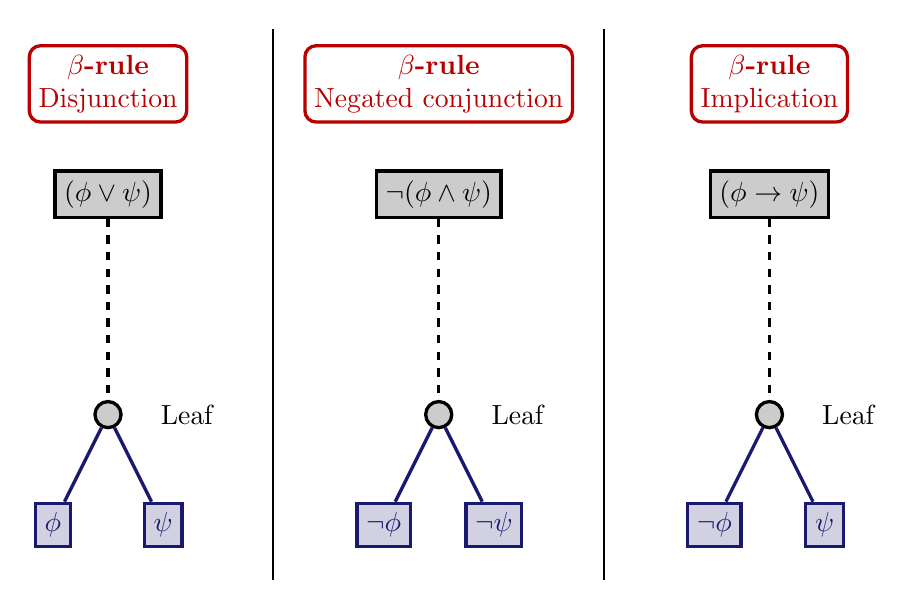
\begin{tikzpicture}[scale=1.4]
        \begin{scope}[shift={(0, 0)}]
            \node (root) at (0, 1)[draw=BrickRed, very thick, BrickRed, rounded corners, align=center] {\textbf{\(\beta\)-rule} \\ Disjunction};

            \node (root) at (0, 0)[draw=black, very thick, fill=black!20] {\((\phi\lor\psi)\)};

            \node (leaf) at (0, -2)[circle, draw=black, very thick, fill=black!20] {};

            \node [right of=leaf, black] {Leaf};

            \draw[dashed, very thick] (root) -- (leaf);

            \node (child1) at (-0.5, -3)[draw=MidnightBlue, very thick, MidnightBlue, fill=MidnightBlue!20] {\(\phi\)};

            \node (child2) at (0.5, -3)[draw=MidnightBlue, very thick, MidnightBlue, fill=MidnightBlue!20] {\(\psi\)};

            \draw[very thick, MidnightBlue] (leaf) -- (child1);
            \draw[very thick, MidnightBlue] (leaf) -- (child2);
        \end{scope}

        \begin{scope}[shift={(3, 0)}]
            \node (root) at (0, 1)[draw=BrickRed, very thick, BrickRed, rounded corners, align=center] {\textbf{\(\beta\)-rule} \\ Negated conjunction};

            \node (root) at (0, 0)[draw=black, very thick, fill=black!20] {\(\neg(\phi\land\psi)\)};

            \node (leaf) at (0, -2)[circle, draw=black, very thick, fill=black!20] {};

            \node [right of=leaf, black] {Leaf};

            \draw[dashed, very thick] (root) -- (leaf);

            \node (child1) at (-0.5, -3)[draw=MidnightBlue, very thick, MidnightBlue, fill=MidnightBlue!20] {\(\neg\phi\)};

            \node (child2) at (0.5, -3)[draw=MidnightBlue, very thick, MidnightBlue, fill=MidnightBlue!20] {\(\neg\psi\)};

            \draw[very thick, MidnightBlue] (leaf) -- (child1);
            \draw[very thick, MidnightBlue] (leaf) -- (child2);
        \end{scope}

        \begin{scope}[shift={(6, 0)}]
            \node (root) at (0, 1)[draw=BrickRed, very thick, BrickRed, rounded corners, align=center] {\textbf{\(\beta\)-rule} \\ Implication};

            \node (root) at (0, 0)[draw=black, very thick, fill=black!20] {\((\phi\rightarrow\psi)\)};

            \node (leaf) at (0, -2)[circle, draw=black, very thick, fill=black!20] {};

            \node [right of=leaf, black] {Leaf};

            \draw[dashed, very thick] (root) -- (leaf);

            \node (child1) at (-0.5, -3)[draw=MidnightBlue, very thick, MidnightBlue, fill=MidnightBlue!20] {\(\neg\phi\)};

            \node (child2) at (0.5, -3)[draw=MidnightBlue, very thick, MidnightBlue, fill=MidnightBlue!20] {\(\psi\)};

            \draw[very thick, MidnightBlue] (leaf) -- (child1);
            \draw[very thick, MidnightBlue] (leaf) -- (child2);
        \end{scope}
        
        \foreach \x in {1.5, 4.5} {
            \draw[thick] (\x, 1.5) -- (\x, -3.5);
        }
    \end{tikzpicture}
    \caption{The three \(\beta\)-rules for constructing propositional tableaus.}
    \label{fig:Ch03-beta-rules}
\end{figure}

In general, nodes located in the same branch\footnote{A \emph{branch} is defined as a path from the root of the tableau to one of its leaves.} are considered in conjunction while the different branches are considered to be disjuncted. As a result, a tableau is a tree-like representation of a formula that is a disjunction of conjunctions, à la disjunctive normal form (DNF).

A tableau is considered \emph{complete} if every node is either ticked (already expanded) or a literal. When a tableau is complete, we can determine the original formula's satisfiability as follows.
%
\begin{itemize}
    \item A branch containing both a propositional letter and its negation (\(p\) and \(\neg p\)) is said to be \emph{closed}, which we denote as \(\oplus\). Otherwise, it is \emph{open}.
    \item A tableau where all branches are closed is said to be \emph{closed}, meaning that the formula at its root is unsatisfiable. Contrarily, a tableau with at least one open branch is said to be \emph{open}, indicating that the formula is satisfiable.
\end{itemize}



\subsection{Example of constructing a tableau and converting to DNF}

To check if the formula
%
\[((p \lor q) \land (\neg p \rightarrow \neg q))\]
%
is satisfiable, we construct its tableau, as shown in figure \ref{fig:Ch03-satisfiability-tableau}.

Since only one of the four branches is closed, this formula is satisfiable. In fact, the literals in each open branch give a possible valuation that satisfies the given formula. For instance, the second branch from the left contains the literals \(p\) and \(\neg q\). This indicates that the formula is true when \(p\) is true and \(q\) is false.

\begin{figure}[H]
    \centering
    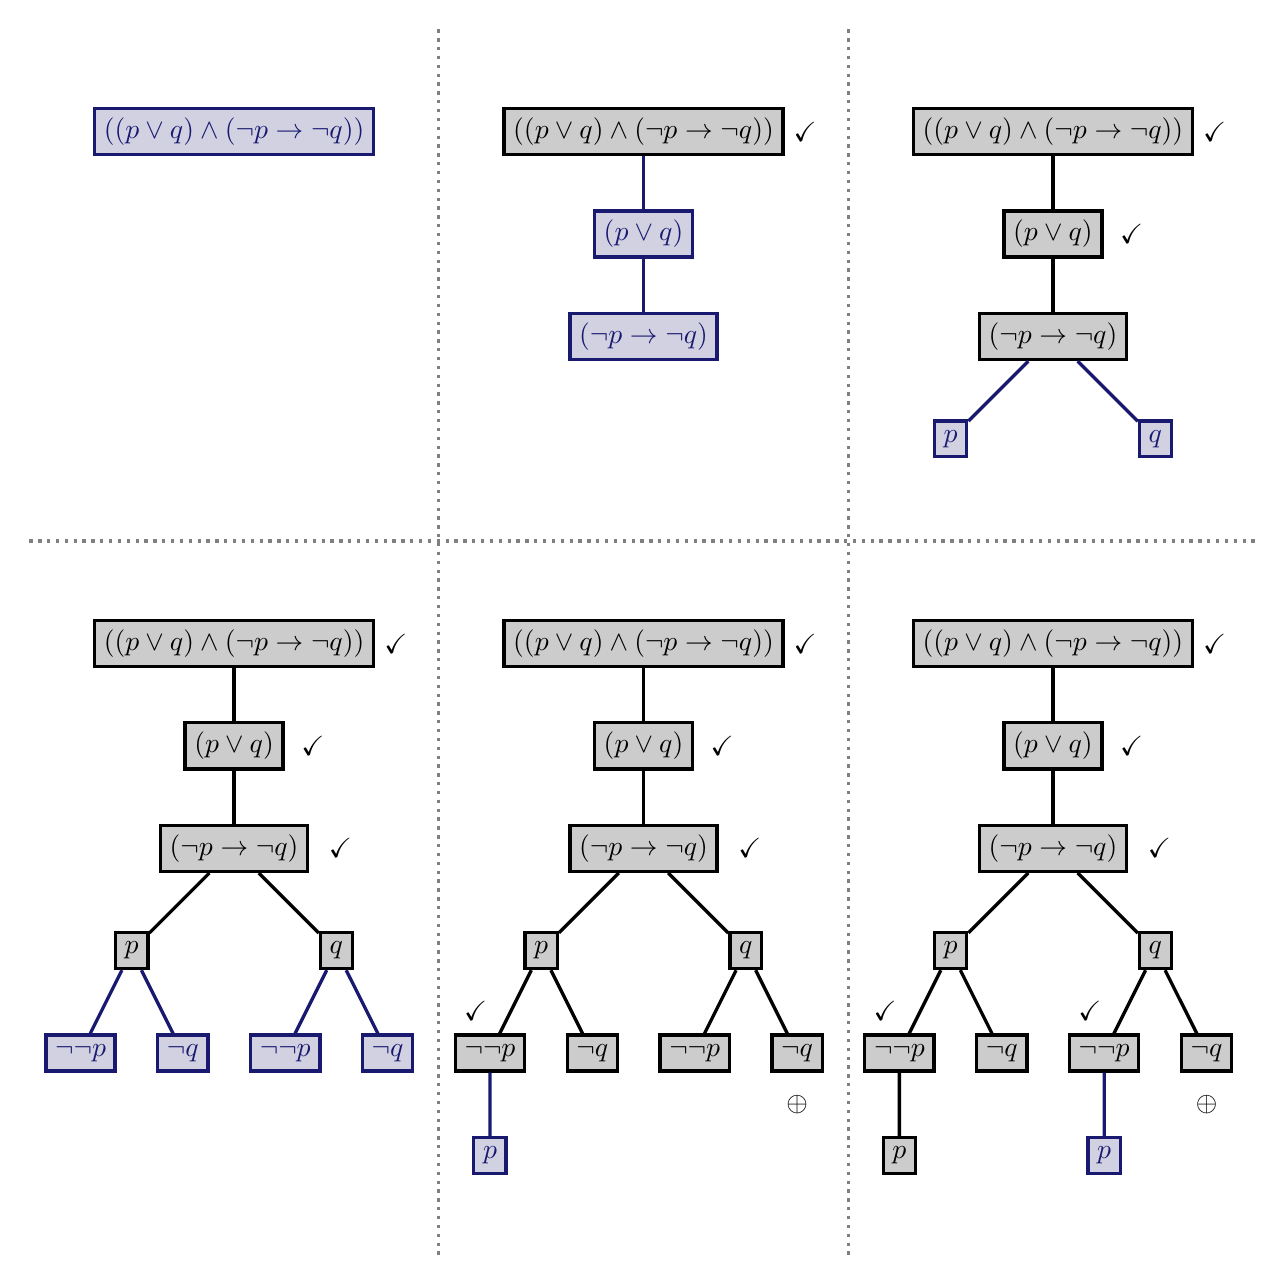
\begin{tikzpicture}[scale=1.3]
        \begin{scope}[shift={(0, 0)}]
            \node (0) at (0, 0)[draw=MidnightBlue, very thick, MidnightBlue, fill=MidnightBlue!20] {\(((p \lor q) \land (\neg p \rightarrow \neg q))\)};
        \end{scope}

        \begin{scope}[shift={(4, 0)}]
            \node (0) at (0, 0)[draw=black, very thick, fill=black!20] {\(((p \lor q) \land (\neg p \rightarrow \neg q))\)};
            \node[right of=0, xshift=30pt] {\checkmark};

            \node (1) at (0, -1)[draw=MidnightBlue, very thick, MidnightBlue, fill=MidnightBlue!20] {\((p \lor q)\)};

            \node (2) at (0, -2)[draw=MidnightBlue, very thick, MidnightBlue, fill=MidnightBlue!20] {\((\neg p \rightarrow \neg q)\)};

            \draw[MidnightBlue, very thick] (0) -- (1) -- (2);
        \end{scope}

        \begin{scope}[shift={(8, 0)}]
            \node (0) at (0, 0)[draw=black, very thick, fill=black!20] {\(((p \lor q) \land (\neg p \rightarrow \neg q))\)};
            \node[right of=0, xshift=30pt] {\checkmark};

            \node (1) at (0, -1)[draw=black, very thick, fill=black!20] {\((p \lor q)\)};
            \node[right of=1] {\checkmark};

            \node (2) at (0, -2)[draw=black, very thick, fill=black!20] {\((\neg p \rightarrow \neg q)\)};

            \node (3) at (-1, -3)[draw=MidnightBlue, very thick, MidnightBlue, fill=MidnightBlue!20] {\(p\)};

            \node (4) at (1, -3)[draw=MidnightBlue, very thick, MidnightBlue, fill=MidnightBlue!20] {\(q\)};

            \draw[black, very thick] (0) -- (1) -- (2);
            \draw[MidnightBlue, very thick] (2) -- (3);
            \draw[MidnightBlue, very thick] (2) -- (4);
        \end{scope}

        \begin{scope}[shift={(0, -5)}]
            \node (0) at (0, 0)[draw=black, very thick, fill=black!20] {\(((p \lor q) \land (\neg p \rightarrow \neg q))\)};
            \node[right of=0, xshift=30pt] {\checkmark};

            \node (1) at (0, -1)[draw=black, very thick, fill=black!20] {\((p \lor q)\)};
            \node[right of=1] {\checkmark};

            \node (2) at (0, -2)[draw=black, very thick, fill=black!20] {\((\neg p \rightarrow \neg q)\)};
            \node[right of=2, xshift=10pt] {\checkmark};

            \node (3) at (-1, -3)[draw=black, very thick, fill=black!20] {\(p\)};

            \node (4) at (1, -3)[draw=black, very thick, fill=black!20] {\(q\)};

            \node (5) at (-1.5, -4)[draw=MidnightBlue, very thick, MidnightBlue, fill=MidnightBlue!20] {\(\neg\neg p\)};

            \node (6) at (-0.5, -4)[draw=MidnightBlue, very thick, MidnightBlue, fill=MidnightBlue!20] {\(\neg q\)};

            \node (7) at (0.5, -4)[draw=MidnightBlue, very thick, MidnightBlue, fill=MidnightBlue!20] {\(\neg\neg p\)};

            \node (8) at (1.5, -4)[draw=MidnightBlue, very thick, MidnightBlue, fill=MidnightBlue!20] {\(\neg q\)};

            \draw[black, very thick] (0) -- (1) -- (2);
            \draw[black, very thick] (2) -- (3);
            \draw[black, very thick] (2) -- (4);
            \draw[MidnightBlue, very thick] (3) -- (5);
            \draw[MidnightBlue, very thick] (3) -- (6);
            \draw[MidnightBlue, very thick] (4) -- (7);
            \draw[MidnightBlue, very thick] (4) -- (8);
        \end{scope}

        \begin{scope}[shift={(4, -5)}]
            \node (0) at (0, 0)[draw=black, very thick, fill=black!20] {\(((p \lor q) \land (\neg p \rightarrow \neg q))\)};
            \node[right of=0, xshift=30pt] {\checkmark};

            \node (1) at (0, -1)[draw=black, very thick, fill=black!20] {\((p \lor q)\)};
            \node[right of=1] {\checkmark};

            \node (2) at (0, -2)[draw=black, very thick, fill=black!20] {\((\neg p \rightarrow \neg q)\)};
            \node[right of=2, xshift=10pt] {\checkmark};

            \node (3) at (-1, -3)[draw=black, very thick, fill=black!20] {\(p\)};

            \node (4) at (1, -3)[draw=black, very thick, fill=black!20] {\(q\)};

            \node (5) at (-1.5, -4)[draw=black, very thick, fill=black!20] {\(\neg\neg p\)};
            \node[above left of=5, xshift=15pt, yshift=-5pt] {\checkmark};

            \node (6) at (-0.5, -4)[draw=black, very thick, fill=black!20] {\(\neg q\)};

            \node (7) at (0.5, -4)[draw=black, very thick, fill=black!20] {\(\neg\neg p\)};

            \node (8) at (1.5, -4)[draw=black, very thick, fill=black!20] {\(\neg q\)};
            \node [below of=8, yshift=10pt] {\(\oplus\)};
            
            \node (9) at (-1.5, -5)[draw=MidnightBlue, very thick, MidnightBlue, fill=MidnightBlue!20] {\(p\)};

            \draw[black, very thick] (0) -- (1) -- (2);
            \draw[black, very thick] (2) -- (3);
            \draw[black, very thick] (2) -- (4);
            \draw[black, very thick] (3) -- (5);
            \draw[black, very thick] (3) -- (6);
            \draw[black, very thick] (4) -- (7);
            \draw[black, very thick] (4) -- (8);
            \draw[MidnightBlue, very thick] (5) -- (9);
        \end{scope}

        \begin{scope}[shift={(8, -5)}]
            \node (0) at (0, 0)[draw=black, very thick, fill=black!20] {\(((p \lor q) \land (\neg p \rightarrow \neg q))\)};
            \node[right of=0, xshift=30pt] {\checkmark};

            \node (1) at (0, -1)[draw=black, very thick, fill=black!20] {\((p \lor q)\)};
            \node[right of=1] {\checkmark};

            \node (2) at (0, -2)[draw=black, very thick, fill=black!20] {\((\neg p \rightarrow \neg q)\)};
            \node[right of=2, xshift=10pt] {\checkmark};

            \node (3) at (-1, -3)[draw=black, very thick, fill=black!20] {\(p\)};

            \node (4) at (1, -3)[draw=black, very thick, fill=black!20] {\(q\)};

            \node (5) at (-1.5, -4)[draw=black, very thick, fill=black!20] {\(\neg\neg p\)};
            \node[above left of=5, xshift=15pt, yshift=-5pt] {\checkmark};

            \node (6) at (-0.5, -4)[draw=black, very thick, fill=black!20] {\(\neg q\)};

            \node (7) at (0.5, -4)[draw=black, very thick, fill=black!20] {\(\neg\neg p\)};
            \node[above left of=7, xshift=15pt, yshift=-5pt] {\checkmark};

            \node (8) at (1.5, -4)[draw=black, very thick, fill=black!20] {\(\neg q\)};
            \node [below of=8, yshift=10pt] {\(\oplus\)};
            
            \node (9) at (-1.5, -5)[draw=black, very thick, fill=black!20] {\(p\)};

            \node (10) at (0.5, -5)[draw=MidnightBlue, very thick, MidnightBlue, fill=MidnightBlue!20] {\(p\)};

            \draw[black, very thick] (0) -- (1) -- (2);
            \draw[black, very thick] (2) -- (3);
            \draw[black, very thick] (2) -- (4);
            \draw[black, very thick] (3) -- (5);
            \draw[black, very thick] (3) -- (6);
            \draw[black, very thick] (4) -- (7);
            \draw[black, very thick] (4) -- (8);
            \draw[black, very thick] (5) -- (9);
            \draw[MidnightBlue, very thick] (7) -- (10);
        \end{scope}

        \draw[gray, very thick, dotted] (2, 1) -- (2, -11);
        \draw[gray, very thick, dotted] (6, 1) -- (6, -11);
        \draw[gray, very thick, dotted] (-2, -4) -- (10, -4);
    \end{tikzpicture}
    \caption{Constructing the tableau of \(((p \lor q) \land (\neg p \rightarrow \neg q))\). Read from left to right and from top to bottom.}
    \label{fig:Ch03-satisfiability-tableau}
\end{figure}

It follows that given the tableau of a formula, its DNF equivalent can be expressed as
%
\[
    \smashoperator{
        \mathop{
            \mathlarger{\mathlarger{\mathlarger{
                \lor
            }}}
        }
    }_{\text{open branch } \Theta}
    \left(
        \mathlarger{\mathlarger{\mathlarger{
            \land
        }}}
        \;\raisebox{2pt}{\(\{\text{literals in } \Theta\}\)}
    \right)
    \text{.}
\]

As always, the CNF of a formula can be obtained by negating the DNF form of its negation.

\newpage
\section{Predicate tableau}

In first-order logic, a \emph{literal} is an atom or its negation, i.e.
%
\[r^n (t_1, t_2, \cdots, t_n)\]
or
\[\neg r^n (t_1, t_2, \cdots, t_n)\]
%
where \(r^n\) is an \(n\)-ary predicate and \(t_i\) is a term.

The method for tableau construction in first-order logic is identical to that in propositional logic, but with a few extra expansion rules for dealing with quantifiers.


\subsection{Expansion rules}

In addition to \(\alpha\)- and \(\beta\)-rules, we also require \(\delta\)- and \(\gamma\)-rules, as depicted in Figures \ref{fig:Ch04-delta-rules} and \ref{fig:Ch04-gamma-rules}.


\begin{figure}[H]
    \centering
    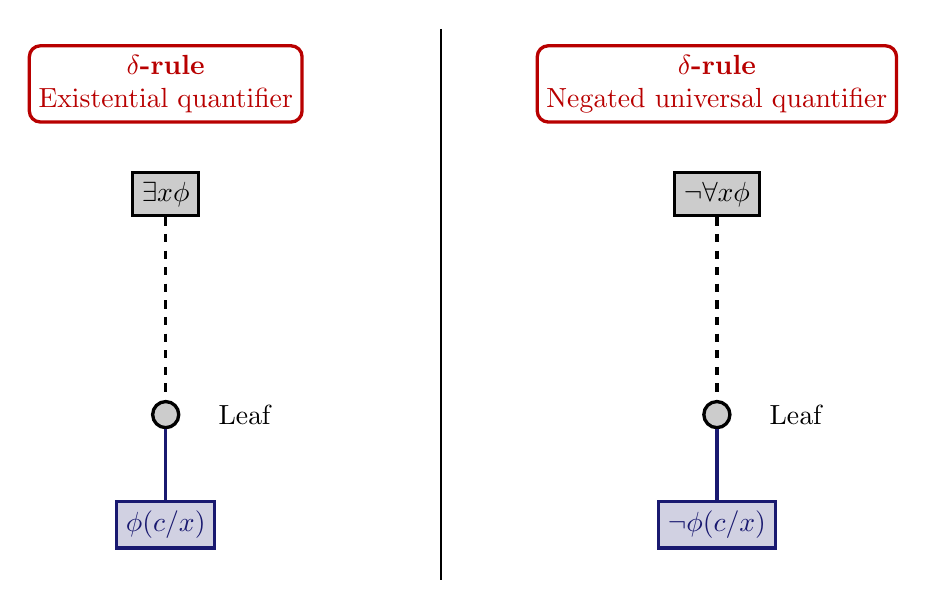
\begin{tikzpicture}[scale=1.4]
        \begin{scope}[shift={(0, 0)}]
            \node (root) at (0, 1)[draw=BrickRed, very thick, BrickRed, rounded corners, align=center] {\textbf{\(\delta\)-rule} \\ Existential quantifier};

            \node (root) at (0, 0)[draw=black, very thick, fill=black!20] {\(\exists x \phi\)};

            \node (leaf) at (0, -2)[circle, draw=black, very thick, fill=black!20] {};

            \node [right of=leaf, black] {Leaf};

            \draw[dashed, very thick] (root) -- (leaf);

            \node (child1) at (0, -3)[draw=MidnightBlue, very thick, MidnightBlue, fill=MidnightBlue!20] {\(\phi(c/ x)\)};

            \draw[very thick, MidnightBlue] (leaf) -- (child1);
        \end{scope}
        
        \begin{scope}[shift={(5, 0)}]
            \node (root) at (0, 1)[draw=BrickRed, very thick, BrickRed, rounded corners, align=center] {\textbf{\(\delta\)-rule} \\ Negated universal quantifier};

            \node (root) at (0, 0)[draw=black, very thick, fill=black!20] {\(\neg\forall x \phi\)};

            \node (leaf) at (0, -2)[circle, draw=black, very thick, fill=black!20] {};

            \node [right of=leaf, black] {Leaf};

            \draw[dashed, very thick] (root) -- (leaf);

            \node (child1) at (0, -3)[draw=MidnightBlue, very thick, MidnightBlue, fill=MidnightBlue!20] {\(\neg\phi(c/ x)\)};

            \draw[very thick, MidnightBlue] (leaf) -- (child1);
        \end{scope}

        \draw[thick] (2.5, 1.5) -- (2.5, -3.5);
    \end{tikzpicture}
    \caption{The two \(\delta\)-rules for constructing predicate tableaus. In both rules, \(c\) should be a new constant that has not been used in the tableau before.}
    \label{fig:Ch04-delta-rules}
\end{figure}


\begin{figure}[H]
    \centering
    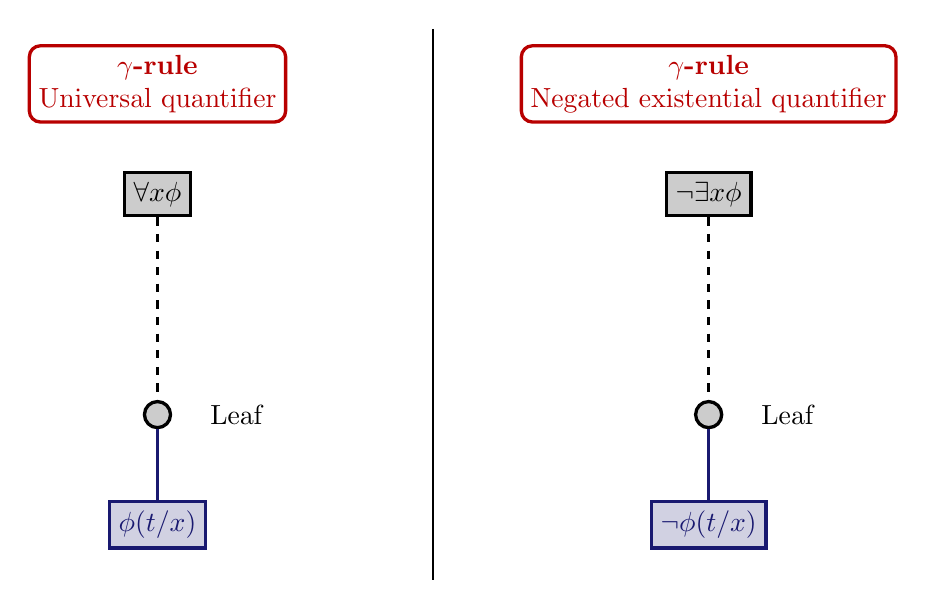
\begin{tikzpicture}[scale=1.4]
        \begin{scope}[shift={(0, 0)}]
            \node (root) at (0, 1)[draw=BrickRed, very thick, BrickRed, rounded corners, align=center] {\textbf{\(\gamma\)-rule} \\ Universal quantifier};

            \node (root) at (0, 0)[draw=black, very thick, fill=black!20] {\(\forall x \phi\)};

            \node (leaf) at (0, -2)[circle, draw=black, very thick, fill=black!20] {};

            \node [right of=leaf, black] {Leaf};

            \draw[dashed, very thick] (root) -- (leaf);

            \node (child1) at (0, -3)[draw=MidnightBlue, very thick, MidnightBlue, fill=MidnightBlue!20] {\(\phi(t/x)\)};

            \draw[very thick, MidnightBlue] (leaf) -- (child1);
        \end{scope}

        \begin{scope}[shift={(5, 0)}]
            \node (root) at (0, 1)[draw=BrickRed, very thick, BrickRed, rounded corners, align=center] {\textbf{\(\gamma\)-rule} \\ Negated existential quantifier};

            \node (root) at (0, 0)[draw=black, very thick, fill=black!20] {\(\neg\exists x \phi\)};

            \node (leaf) at (0, -2)[circle, draw=black, very thick, fill=black!20] {};

            \node [right of=leaf, black] {Leaf};

            \draw[dashed, very thick] (root) -- (leaf);

            \node (child1) at (0, -3)[draw=MidnightBlue, very thick, MidnightBlue, fill=MidnightBlue!20] {\(\neg\phi(t/ x)\)};

            \draw[very thick, MidnightBlue] (leaf) -- (child1);
        \end{scope}

        \draw[thick] (2.5, 1.5) -- (2.5, -3.5);
    \end{tikzpicture}
    \caption{The two \(\gamma\)-rules for constructing predicate tableaus. In both rules, \(t\) is a closed term. Formulas should \textbf{not} be ticked following a \(\gamma\)-rule expansion.}
    \label{fig:Ch04-gamma-rules}
\end{figure}

When applying a \(\delta\)-rule, make sure to introduce a new constant symbol that is not used anywhere before in the tableau. This new constant acts as a \emph{witness}\footnote{Or: \emph{Skolem witness}.} for the existential statement.

Compared to the other rules, \(\gamma\)-rules are usually applied last. When applying a \(\gamma\)-rule, instantiate \(x\) with a closed term that appeared earlier in the current branch\footnote{This closed term should \textbf{not} be new.}. Formulas expanded via a \(\gamma\)-rule should \textbf{not} be ticked.



\subsection{Termination}

Similar to propositional tableaus, a predicate tableau's branch is closed if it contains both a literal \(P(t_1, t_2, \cdots, t_n)\) and its negation \(\neg P(t_1, t_2, \cdots, t_n)\). Otherwise, it is open.

The tableau terminates when:
%
\begin{itemize}
    \item Every branch is closed. This shows that the root formula is unsatisfiable.
    \item All formulas are fully expanded and no further rules can be applied. If at least one branch remains open and cannot be further expanded, the tableau is open, indicating the root formula's satisfiability.
\end{itemize}




\subsection{Example}

Suppose we want to check whether the formula
%
\[(\forall x\; \neg p(x) \rightarrow \neg\exists y\; p(y))\]
%
is valid. To do this, we place its negation at the root of our tableau.


\begin{figure}[H]
    \centering
    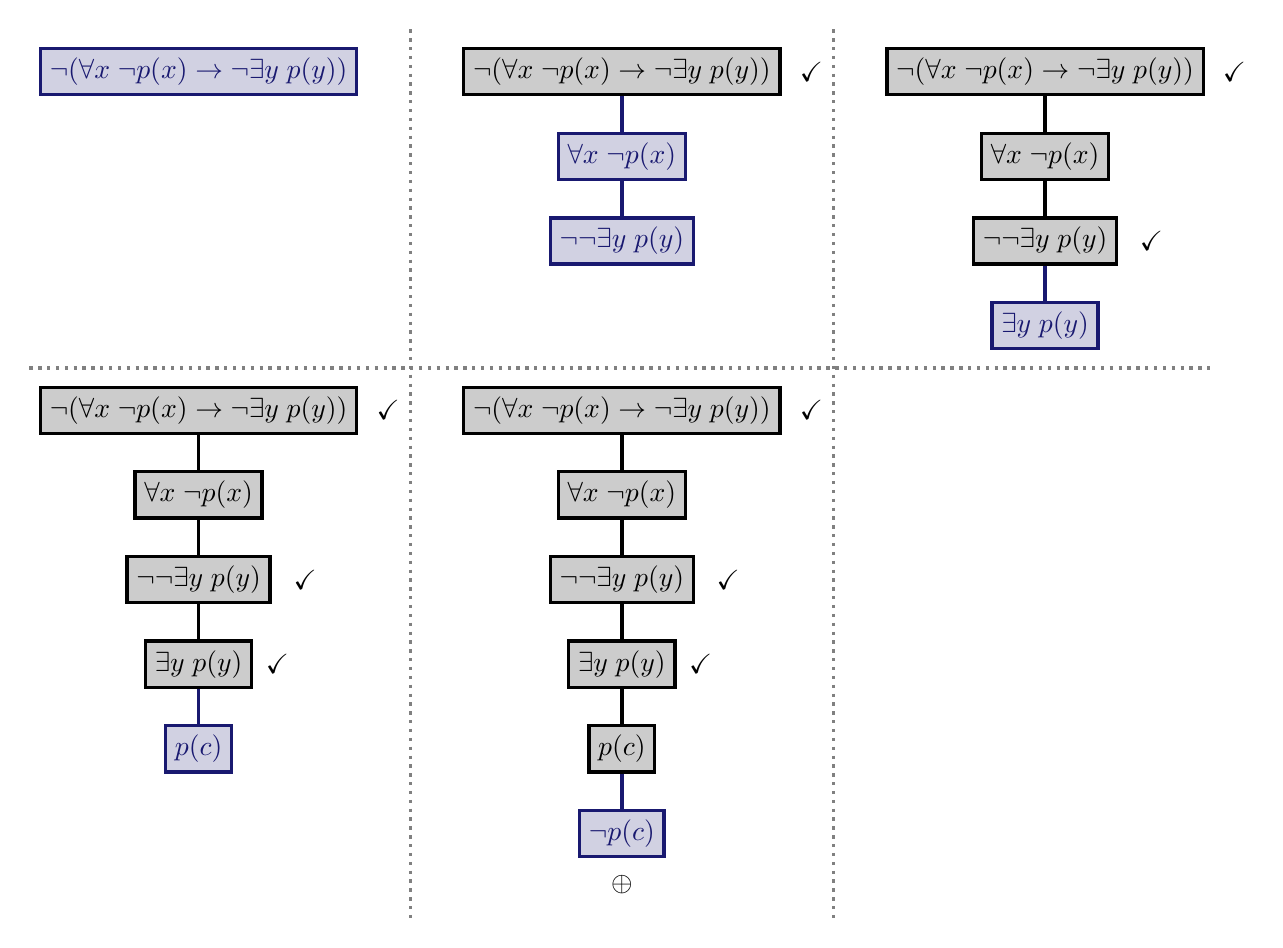
\begin{tikzpicture}[scale=1.075]
        \begin{scope}[shift={(0, 0)}]
            \node (0) at (0, 0)[draw=MidnightBlue, very thick, MidnightBlue, fill=MidnightBlue!20] {\(\neg(\forall x\; \neg p(x) \rightarrow \neg\exists y\; p(y))\)};
        \end{scope}

        \begin{scope}[shift={(5, 0)}]
            \node (0) at (0, 0)[draw=black, very thick, fill=black!20] {\(\neg(\forall x\; \neg p(x) \rightarrow \neg\exists y\; p(y))\)};
            \node[right of=0, xshift=40pt] {\checkmark};

            \node (1) at (0, -1)[draw=MidnightBlue, very thick, MidnightBlue, fill=MidnightBlue!20] {\(\forall x\; \neg p(x)\)};

            \node (2) at (0, -2)[draw=MidnightBlue, very thick, MidnightBlue, fill=MidnightBlue!20] {\(\neg\neg\exists y\; p(y)\)};

            \draw[MidnightBlue, very thick] (0) -- (1) -- (2);
        \end{scope}

        \begin{scope}[shift={(10, 0)}]
            \node (0) at (0, 0)[draw=black, very thick, fill=black!20] {\(\neg(\forall x\; \neg p(x) \rightarrow \neg\exists y\; p(y))\)};
            \node[right of=0, xshift=40pt] {\checkmark};

            \node (1) at (0, -1)[draw=black, very thick, fill=black!20] {\(\forall x\; \neg p(x)\)};

            \node (2) at (0, -2)[draw=black, very thick, fill=black!20] {\(\neg\neg\exists y\; p(y)\)};
            \node[right of=2, xshift=10pt] {\checkmark};

            \node (3) at (0, -3)[draw=MidnightBlue, very thick, MidnightBlue, fill=MidnightBlue!20] {\(\exists y\; p(y)\)};

            \draw[black, very thick] (0) -- (1) -- (2);
            \draw[MidnightBlue, very thick] (2) -- (3);
        \end{scope}

        \begin{scope}[shift={(0, -4)}]
            \node (0) at (0, 0)[draw=black, very thick, fill=black!20] {\(\neg(\forall x\; \neg p(x) \rightarrow \neg\exists y\; p(y))\)};
            \node[right of=0, xshift=40pt] {\checkmark};

            \node (1) at (0, -1)[draw=black, very thick, fill=black!20] {\(\forall x\; \neg p(x)\)};

            \node (2) at (0, -2)[draw=black, very thick, fill=black!20] {\(\neg\neg\exists y\; p(y)\)};
            \node[right of=2, xshift=10pt] {\checkmark};

            \node (3) at (0, -3)[draw=black, very thick, fill=black!20] {\(\exists y\; p(y)\)};
            \node[right of=3] {\checkmark};

            \node (4) at (0, -4)[draw=MidnightBlue, very thick, MidnightBlue, fill=MidnightBlue!20] {\(p(c)\)};

            \draw[black, very thick] (0) -- (1) -- (2) -- (3);
            \draw[MidnightBlue, very thick] (3) -- (4);
        \end{scope}

        \begin{scope}[shift={(5, -4)}]
            \node (0) at (0, 0)[draw=black, very thick, fill=black!20] {\(\neg(\forall x\; \neg p(x) \rightarrow \neg\exists y\; p(y))\)};
            \node[right of=0, xshift=40pt] {\checkmark};

            \node (1) at (0, -1)[draw=black, very thick, fill=black!20] {\(\forall x\; \neg p(x)\)};

            \node (2) at (0, -2)[draw=black, very thick, fill=black!20] {\(\neg\neg\exists y\; p(y)\)};
            \node[right of=2, xshift=10pt] {\checkmark};

            \node (3) at (0, -3)[draw=black, very thick, fill=black!20] {\(\exists y\; p(y)\)};
            \node[right of=3] {\checkmark};

            \node (4) at (0, -4)[draw=black, very thick, fill=black!20] {\(p(c)\)};

            \node (5) at (0, -5)[draw=MidnightBlue, very thick, MidnightBlue, fill=MidnightBlue!20] {\(\neg p(c)\)};
            \node [below of=5, yshift=10pt] {\(\oplus\)};

            \draw[black, very thick] (0) -- (1) -- (2) -- (3) -- (4);
            \draw[MidnightBlue, very thick] (4) -- (5);
        \end{scope}

        \draw[gray, very thick, dotted] (2.5, 0.5) -- (2.5, -10);
        \draw[gray, very thick, dotted] (7.5, 0.5) -- (7.5, -10);
        \draw[gray, very thick, dotted] (-2, -3.5) -- (12, -3.5);
    \end{tikzpicture}
    \caption{Constructing the tableau of \(\neg(\forall x\; \neg p(x) \rightarrow \neg\exists y\; p(y))\). Read from left to right and from top to bottom. In the fourth step (bottom left), the existential formula \(\exists y\; p(y)\) is expanded via a \(\delta\)-rule by introducing a new constant \(c\). In the last step (bottom middle), the universal formula \(\forall x\; \neg p(x)\) is expanded via a \(\gamma\)-rule by replacing all bounded instances of \(x\) with the closed term \(c\) from earlier in the current branch, thereby producing both \(p(c)\) and \(\neg p(c)\) in the same branch. This results in a closed branch and hence a closed tableau, indicating that the formula at the root is unsatisfiable.}
    \label{fig:Ch04-satisfiability-tableau}
\end{figure}

As shown, the negation \(\neg(\forall x\; \neg p(x) \rightarrow \neg\exists y\; p(y))\) is unsatisfiable. This means that our original formula must be valid.




\subsection{Non-termination}

Predicate tableaus may not always terminate.

For instance, if a tableau unendingly generates nodes that require expansion via \(\delta\)-rules, more and more constants would be introduced, and the number of \(\gamma\)-rule applications required would increase dramatically. This may result in non-termination.

Before we elaborate on this non-terminating scenario, we must note that in order to systematically handle possible infinite expansions, we should adopt a fair application strategy. A tableau construction is \emph{fair} if
%
\begin{itemize}
    \item Every formula that can still be expanded eventually will be, and
    \item Every formula that falls under a \(\gamma\)-rule will eventually be instantiated via that rule using all closed terms that appear in its branch.
\end{itemize}
%
This ensures that if the tableau can close, it will close after finitely many steps. We won't miss a contradiction because we ignored a rule.

Now, assuming a fair application strategy,
%
\begin{itemize}
    \item If a branch keeps repeating the same configuration of formulas over and over with no new information, it is effectively saturated. This branch is then considered open, meaning that the root formula is satisfiable. This is because we may construct an infinite model for the root formula by reading off literals in the limit of the infinitely ``looping'' branch in the same way as we did for propositional tableaus. See Figure \ref{fig:Ch04-non-terminating-tableau} for an example.
    \item If a branch runs indefinitely without closure, the satisfiability of the root formula is \textbf{undecided} and \textbf{inconclusive}.
\end{itemize}


\begin{figure}[H]
    \centering
    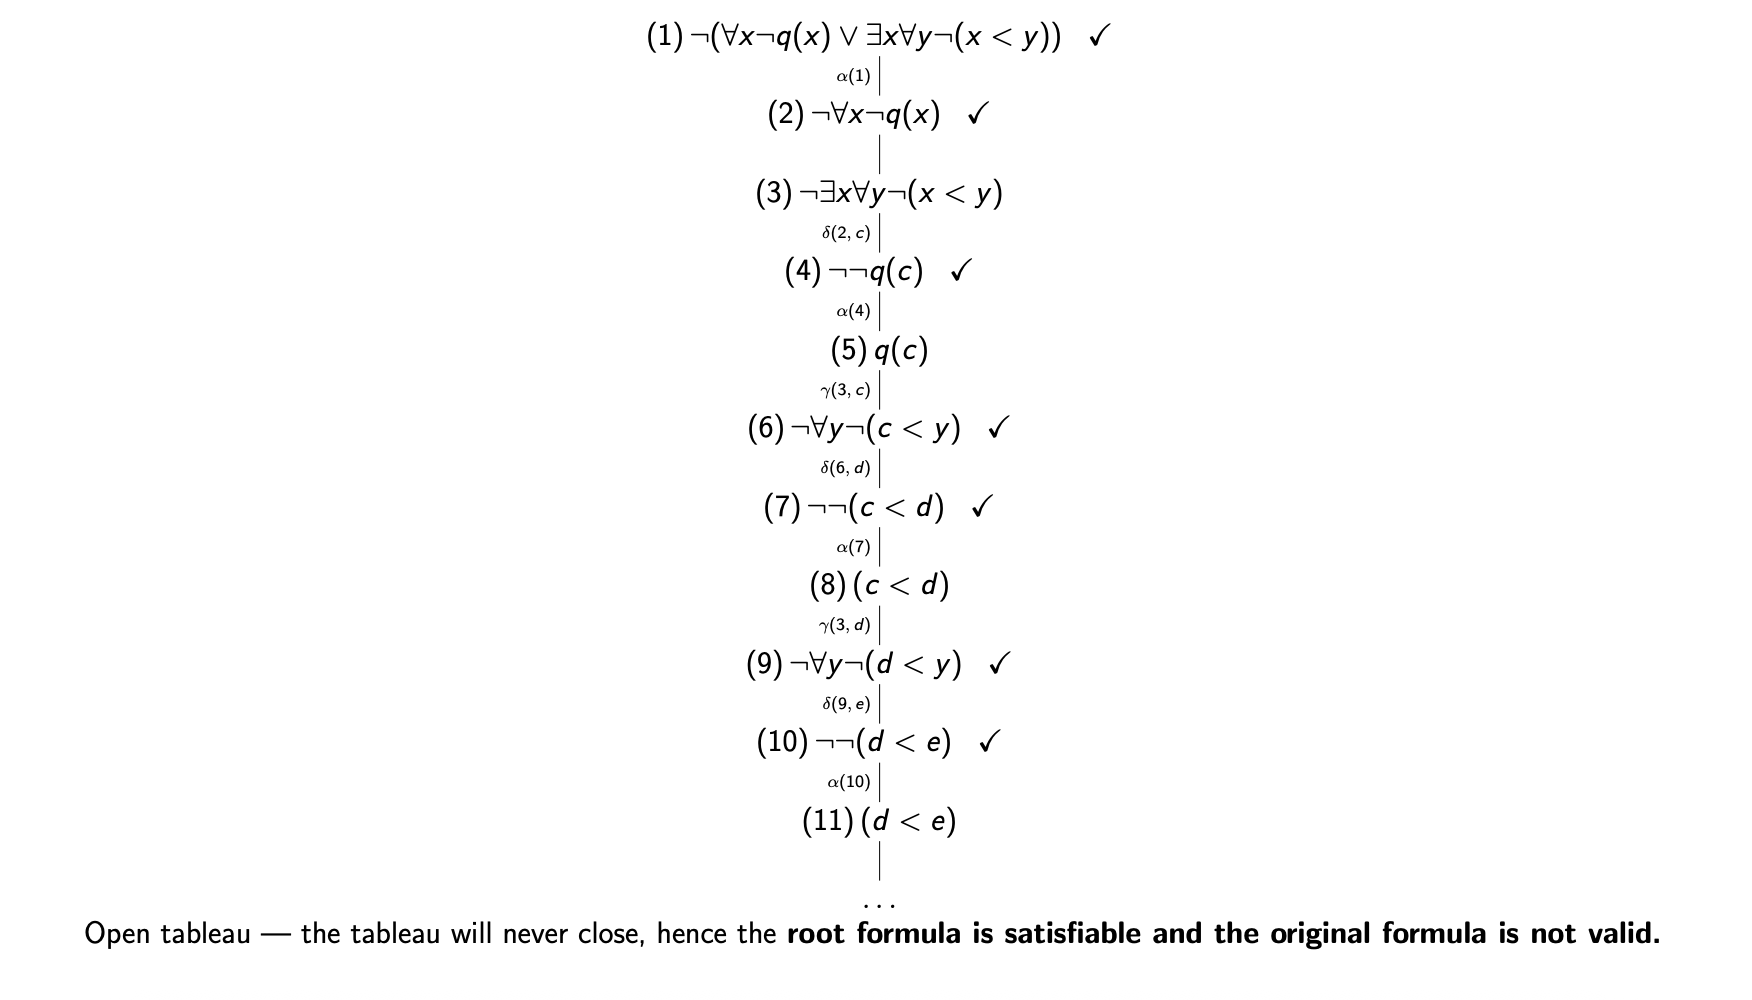
\includegraphics[width=0.95\textwidth]{Images/04a_NonterminatingPredicateTableau.png}
    \caption{A non-terminating tableau where the root formula is satisfiable.}
    \label{fig:Ch04-non-terminating-tableau}
\end{figure}



\subsection{Free variables}

Predicate tableaus are predominantly designed to work on sentences, where free variables are not allowed. To prove the validity of a formula with free variables, we may prefix it with an appropriate universal quantifier. For instance, if we want to show that
%
\[x < 5\]
%
is valid, where \(x\) is a free variable. Notice that this is equivalent to showing the validity of
%
\[\forall x\; x < 5\]
%
which uses a universal quantifier to remove the free variable. Consequently, we can simply construct a tableau with
%
\[\neg\forall x\; x < 5\]
%
at its root and check its satisfiability as usual.



\subsection{More on fairness}

Note that when applying expansion rules in non-terminating predicate tableaus, it is always possible to find a fair application strategy.

To see why this is, consider a countably infinite set of processes \(P = \{P_1, P_2, \cdots, P_i, \cdots\}\), each awaiting some input. When a process receives an input, this may result in the creation of a new process, which is subsequently added to \(P\). We want to find some fair schedule where if any process \(P_i\) is awaiting input at time \(t\), then eventually at some time \(t' > t\) it will receive some input.

Since the set \(P\) always remains countable even when a new process is created and added to it, such a schedule must exist.

\newpage
\section{Proving tableau properties by viewing them as lists}

\subsection{Preliminaries: On subsets and subformulas}

In this subsection, we present two lemmas on subsets and subformulas. Given a formula \(\phi\), a subformula is a substring of \(\phi\) that is also a formula.

\begin{lemma}
    A set \(S\) of cardinality \(n\) has \(2^n\) subsets.
\end{lemma}
\begin{proof}
    To construct a subset \(S' \subseteq S\), each element of \(S\) can either appear or not appear in \(S'\). This involves a total of \(n\) independent binary choices. Hence, there are \(2^n\) possible subsets.
\end{proof}

\begin{lemma}
    A formula \(\phi\) has at most \(\abs{\phi}\) subformulas.
\end{lemma}
\begin{proof}
    Consider the parse tree of \(\phi\), where every node contains exactly one symbol and is the root of a subtree that represents a subformula of \(\phi\). Hence we have
    %
    \begin{align*}
        & \text{Number of subformulas of } \phi\\
        =\;& \text{Number of nodes in parse tree of } \phi\\
        =\;& \text{Number of symbols that appear in parse tree of } \phi\\
        \leq\;& \text{Number of symbols in } \phi \tag{as brackets do not appear in parse trees}\\
        =\;& \abs{\phi}\text{.} \qedhere
    \end{align*}
\end{proof}

\subsection{Tableaus as lists of theories}

While tableaus can be visualised as trees, they can also be represented as lists. To see how this works, let us first review the \(\alpha\)- and \(\beta\)- rules. As shown in tables \ref{tab:Ch05-alpha-rules} and \ref{tab:Ch05-beta-rules}, each \(\alpha\)-rule produces at most two new nodes \(\alpha_1\) and \(\alpha_2\), while each \(\beta\)-rule produces at most two new nodes \(\beta_1\) and \(\beta_2\).

\begin{table}[H]
    \centering
    \begin{tabular}{|c|cc|}
        \hline
        \(\alpha\) & \(\alpha_1\) & \(\alpha_2\)\\
        \hline
        \((A\land B)\) & \(A\) & \(B\)\\
        \hline
        \(\neg(A\lor B)\) & \(\neg A\) & \(\neg B\)\\
        \hline
        \(\neg(A\rightarrow B)\) & \(A\) & \(\neg B\)\\
        \hline
        \(\neg\neg A\) & \(A\) & -\\
        \hline
    \end{tabular}

    \caption{The \(\alpha\)-rules tabulated.}
    \label{tab:Ch05-alpha-rules}
\end{table}

\begin{table}[H]
    \centering
    \begin{tabular}{|c|cc|}
        \hline
        \(\beta\) & \(\beta_1\) & \(\beta_2\)\\
        \hline
        \((A\lor B)\) & \(A\) & \(B\)\\
        \hline
        \((A\rightarrow B)\) & \(\neg A\) & \(B\)\\
        \hline
        \(\neg(A\land B)\) & \(\neg A\) & \(\neg B\)\\
        \hline
    \end{tabular}

    \caption{The \(\beta\)-rules tabulated.}
    \label{tab:Ch05-beta-rules}
\end{table}


Instead of a tree, we represent a tableau as a list of \emph{theories}, where each theory is a set of unticked formulas in a branch that has not yet closed. Figure \ref{fig:Ch05-tableau-as-list}, based on Figure \ref{fig:Ch03-satisfiability-tableau}, shows the construction of a propositional tableau in both tree and list form.


\begin{figure}[H]
    \centering
    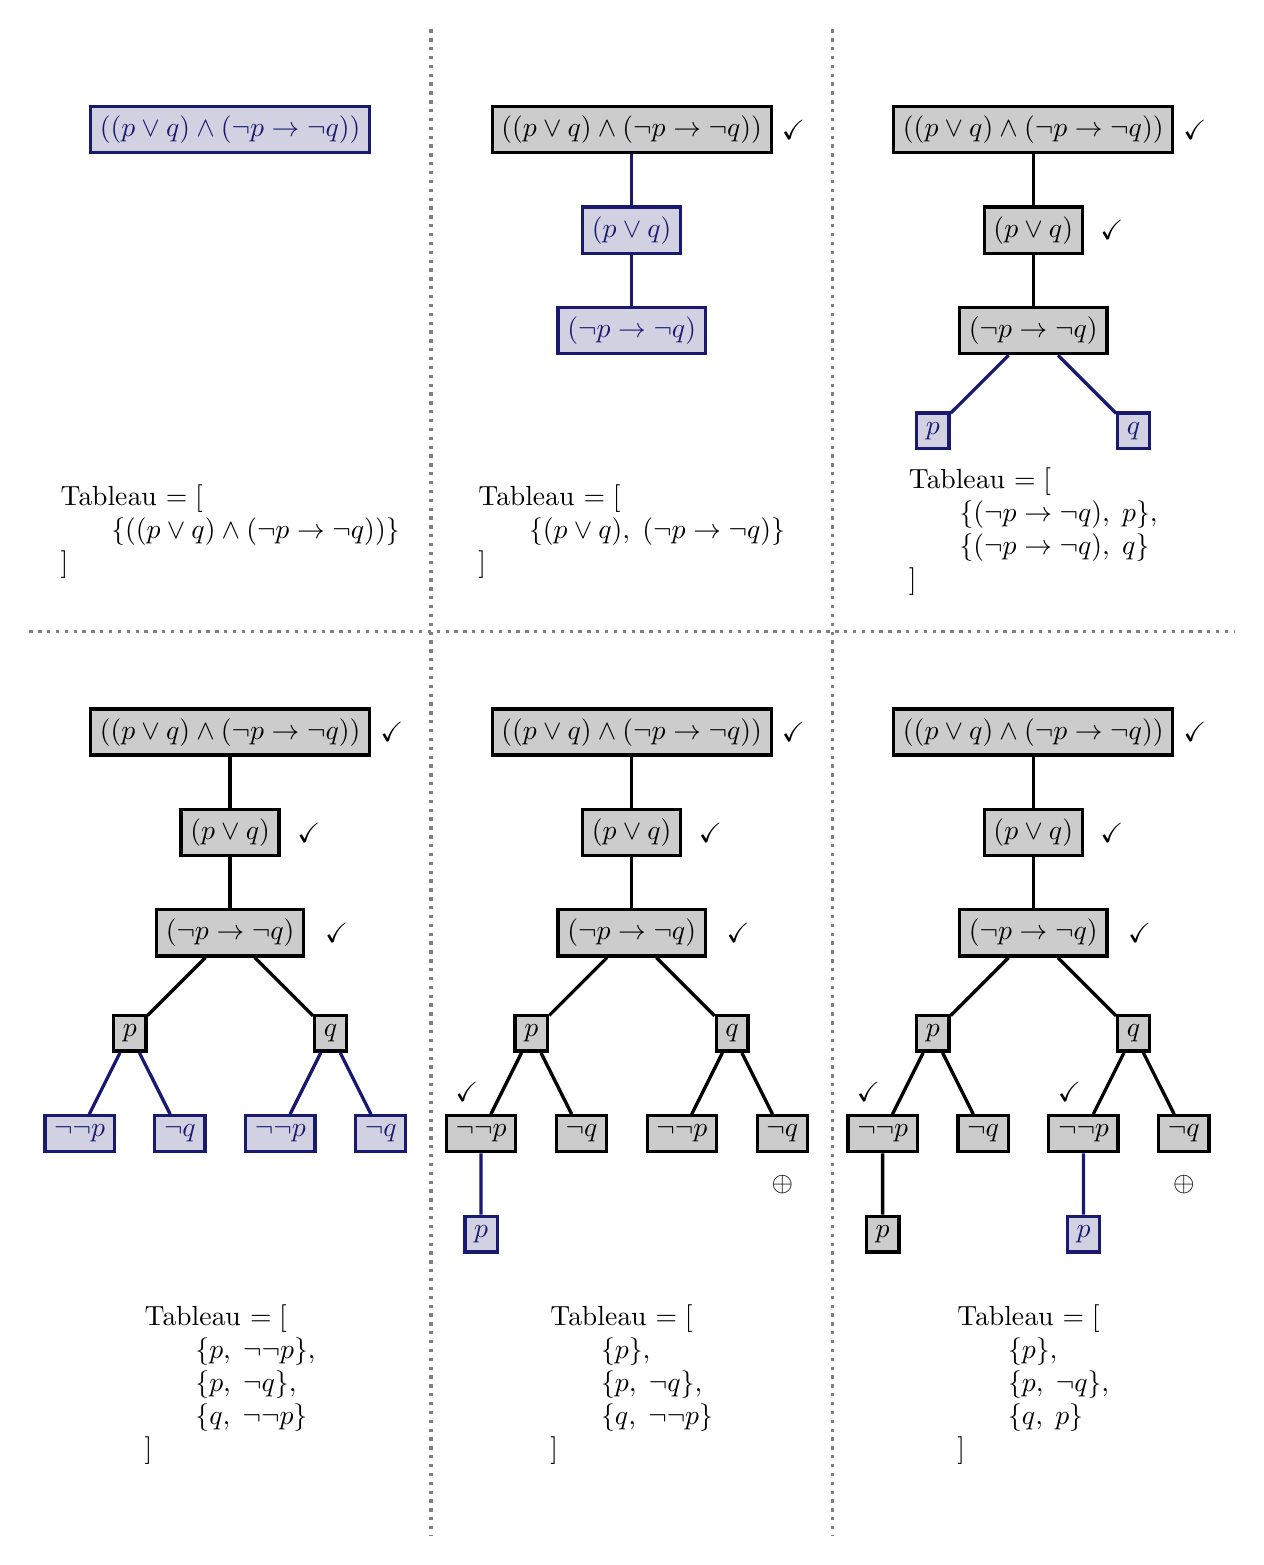
\begin{tikzpicture}[scale=1.275]
        \begin{scope}[shift={(0, 0)}]
            \node (0) at (0, 0)[draw=MidnightBlue, very thick, MidnightBlue, fill=MidnightBlue!20] {\(((p \lor q) \land (\neg p \rightarrow \neg q))\)};

            \node at (0, -4) [black, align=left]{
                Tableau \(= [\)\\
                \hspace{1.5em} \(\{((p \lor q) \land (\neg p \rightarrow \neg q))\}\)\\
                \(]\)
            };
        \end{scope}

        \begin{scope}[shift={(4, 0)}]
            \node (0) at (0, 0)[draw=black, very thick, fill=black!20] {\(((p \lor q) \land (\neg p \rightarrow \neg q))\)};
            \node[right of=0, xshift=30pt] {\checkmark};

            \node (1) at (0, -1)[draw=MidnightBlue, very thick, MidnightBlue, fill=MidnightBlue!20] {\((p \lor q)\)};

            \node (2) at (0, -2)[draw=MidnightBlue, very thick, MidnightBlue, fill=MidnightBlue!20] {\((\neg p \rightarrow \neg q)\)};

            \draw[MidnightBlue, very thick] (0) -- (1) -- (2);

            \node at (0, -4) [black, align=left]{
                Tableau \(= [\)\\
                \hspace{1.5em} \(\{(p \lor q),\; (\neg p \rightarrow \neg q)\}\)\\
                \(]\)
            };
        \end{scope}

        \begin{scope}[shift={(8, 0)}]
            \node (0) at (0, 0)[draw=black, very thick, fill=black!20] {\(((p \lor q) \land (\neg p \rightarrow \neg q))\)};
            \node[right of=0, xshift=30pt] {\checkmark};

            \node (1) at (0, -1)[draw=black, very thick, fill=black!20] {\((p \lor q)\)};
            \node[right of=1] {\checkmark};

            \node (2) at (0, -2)[draw=black, very thick, fill=black!20] {\((\neg p \rightarrow \neg q)\)};

            \node (3) at (-1, -3)[draw=MidnightBlue, very thick, MidnightBlue, fill=MidnightBlue!20] {\(p\)};

            \node (4) at (1, -3)[draw=MidnightBlue, very thick, MidnightBlue, fill=MidnightBlue!20] {\(q\)};

            \draw[black, very thick] (0) -- (1) -- (2);
            \draw[MidnightBlue, very thick] (2) -- (3);
            \draw[MidnightBlue, very thick] (2) -- (4);

            \node at (0, -4) [black, align=left]{
                Tableau \(= [\)\\
                \hspace{1.5em} \(\{(\neg p \rightarrow \neg q),\; p\},\)\\
                \hspace{1.5em} \(\{(\neg p \rightarrow \neg q),\; q\}\)\\
                \(]\)
            };
        \end{scope}

        \begin{scope}[shift={(0, -6)}]
            \node (0) at (0, 0)[draw=black, very thick, fill=black!20] {\(((p \lor q) \land (\neg p \rightarrow \neg q))\)};
            \node[right of=0, xshift=30pt] {\checkmark};

            \node (1) at (0, -1)[draw=black, very thick, fill=black!20] {\((p \lor q)\)};
            \node[right of=1] {\checkmark};

            \node (2) at (0, -2)[draw=black, very thick, fill=black!20] {\((\neg p \rightarrow \neg q)\)};
            \node[right of=2, xshift=10pt] {\checkmark};

            \node (3) at (-1, -3)[draw=black, very thick, fill=black!20] {\(p\)};

            \node (4) at (1, -3)[draw=black, very thick, fill=black!20] {\(q\)};

            \node (5) at (-1.5, -4)[draw=MidnightBlue, very thick, MidnightBlue, fill=MidnightBlue!20] {\(\neg\neg p\)};

            \node (6) at (-0.5, -4)[draw=MidnightBlue, very thick, MidnightBlue, fill=MidnightBlue!20] {\(\neg q\)};

            \node (7) at (0.5, -4)[draw=MidnightBlue, very thick, MidnightBlue, fill=MidnightBlue!20] {\(\neg\neg p\)};

            \node (8) at (1.5, -4)[draw=MidnightBlue, very thick, MidnightBlue, fill=MidnightBlue!20] {\(\neg q\)};

            \draw[black, very thick] (0) -- (1) -- (2);
            \draw[black, very thick] (2) -- (3);
            \draw[black, very thick] (2) -- (4);
            \draw[MidnightBlue, very thick] (3) -- (5);
            \draw[MidnightBlue, very thick] (3) -- (6);
            \draw[MidnightBlue, very thick] (4) -- (7);
            \draw[MidnightBlue, very thick] (4) -- (8);

            \node at (0, -6.5) [black, align=left]{
                Tableau \(= [\)\\
                \hspace{1.5em} \(\{p,\; \neg\neg p\},\)\\
                \hspace{1.5em} \(\{p,\; \neg q\},\)\\
                \hspace{1.5em} \(\{q,\; \neg\neg p\}\)\\
                \(]\)
            };
        \end{scope}

        \begin{scope}[shift={(4, -6)}]
            \node (0) at (0, 0)[draw=black, very thick, fill=black!20] {\(((p \lor q) \land (\neg p \rightarrow \neg q))\)};
            \node[right of=0, xshift=30pt] {\checkmark};

            \node (1) at (0, -1)[draw=black, very thick, fill=black!20] {\((p \lor q)\)};
            \node[right of=1] {\checkmark};

            \node (2) at (0, -2)[draw=black, very thick, fill=black!20] {\((\neg p \rightarrow \neg q)\)};
            \node[right of=2, xshift=10pt] {\checkmark};

            \node (3) at (-1, -3)[draw=black, very thick, fill=black!20] {\(p\)};

            \node (4) at (1, -3)[draw=black, very thick, fill=black!20] {\(q\)};

            \node (5) at (-1.5, -4)[draw=black, very thick, fill=black!20] {\(\neg\neg p\)};
            \node[above left of=5, xshift=15pt, yshift=-5pt] {\checkmark};

            \node (6) at (-0.5, -4)[draw=black, very thick, fill=black!20] {\(\neg q\)};

            \node (7) at (0.5, -4)[draw=black, very thick, fill=black!20] {\(\neg\neg p\)};

            \node (8) at (1.5, -4)[draw=black, very thick, fill=black!20] {\(\neg q\)};
            \node [below of=8, yshift=10pt] {\(\oplus\)};
            
            \node (9) at (-1.5, -5)[draw=MidnightBlue, very thick, MidnightBlue, fill=MidnightBlue!20] {\(p\)};

            \draw[black, very thick] (0) -- (1) -- (2);
            \draw[black, very thick] (2) -- (3);
            \draw[black, very thick] (2) -- (4);
            \draw[black, very thick] (3) -- (5);
            \draw[black, very thick] (3) -- (6);
            \draw[black, very thick] (4) -- (7);
            \draw[black, very thick] (4) -- (8);
            \draw[MidnightBlue, very thick] (5) -- (9);

            \node at (0, -6.5) [black, align=left]{
                Tableau \(= [\)\\
                \hspace{1.5em} \(\{p\},\)\\
                \hspace{1.5em} \(\{p,\; \neg q\},\)\\
                \hspace{1.5em} \(\{q,\; \neg\neg p\}\)\\
                \(]\)
            };
        \end{scope}

        \begin{scope}[shift={(8, -6)}]
            \node (0) at (0, 0)[draw=black, very thick, fill=black!20] {\(((p \lor q) \land (\neg p \rightarrow \neg q))\)};
            \node[right of=0, xshift=30pt] {\checkmark};

            \node (1) at (0, -1)[draw=black, very thick, fill=black!20] {\((p \lor q)\)};
            \node[right of=1] {\checkmark};

            \node (2) at (0, -2)[draw=black, very thick, fill=black!20] {\((\neg p \rightarrow \neg q)\)};
            \node[right of=2, xshift=10pt] {\checkmark};

            \node (3) at (-1, -3)[draw=black, very thick, fill=black!20] {\(p\)};

            \node (4) at (1, -3)[draw=black, very thick, fill=black!20] {\(q\)};

            \node (5) at (-1.5, -4)[draw=black, very thick, fill=black!20] {\(\neg\neg p\)};
            \node[above left of=5, xshift=15pt, yshift=-5pt] {\checkmark};

            \node (6) at (-0.5, -4)[draw=black, very thick, fill=black!20] {\(\neg q\)};

            \node (7) at (0.5, -4)[draw=black, very thick, fill=black!20] {\(\neg\neg p\)};
            \node[above left of=7, xshift=15pt, yshift=-5pt] {\checkmark};

            \node (8) at (1.5, -4)[draw=black, very thick, fill=black!20] {\(\neg q\)};
            \node [below of=8, yshift=10pt] {\(\oplus\)};
            
            \node (9) at (-1.5, -5)[draw=black, very thick, fill=black!20] {\(p\)};

            \node (10) at (0.5, -5)[draw=MidnightBlue, very thick, MidnightBlue, fill=MidnightBlue!20] {\(p\)};

            \draw[black, very thick] (0) -- (1) -- (2);
            \draw[black, very thick] (2) -- (3);
            \draw[black, very thick] (2) -- (4);
            \draw[black, very thick] (3) -- (5);
            \draw[black, very thick] (3) -- (6);
            \draw[black, very thick] (4) -- (7);
            \draw[black, very thick] (4) -- (8);
            \draw[black, very thick] (5) -- (9);
            \draw[MidnightBlue, very thick] (7) -- (10);

            \node at (0, -6.5) [black, align=left]{
                Tableau \(= [\)\\
                \hspace{1.5em} \(\{p\},\)\\
                \hspace{1.5em} \(\{p,\; \neg q\},\)\\
                \hspace{1.5em} \(\{q,\; p\}\)\\
                \(]\)
            };
        \end{scope}

        \draw[gray, very thick, dotted] (2, 1) -- (2, -14);
        \draw[gray, very thick, dotted] (6, 1) -- (6, -14);
        \draw[gray, very thick, dotted] (-2, -5) -- (10, -5);
    \end{tikzpicture}
    \caption{Constructing the tableau of \(((p \lor q) \land (\neg p \rightarrow \neg q))\) as a tree and as a list. Read from left to right and from top to bottom.}
    \label{fig:Ch05-tableau-as-list}
\end{figure}


\newpage
Below is a pseudocode snippet outlining how the propositional tableau method can be implemented programmatically using the list representation. Here, \verb|Tableau| is initialised as a queue of theories. The variables \(\alpha_1\), \(\alpha_2\), \(\beta_1\) and \(\beta_2\) refer to the ones labelled in Tables \ref{tab:Ch05-alpha-rules} and \ref{tab:Ch05-beta-rules}.


\begin{lstlisting}[language=python, commentstyle=\color{gray}]
def is_satisfiable($\phi$):
    Tableau = Queue()
    Tableau.enqueue($\phi$)

    while Tableau is not empty:
        # Dequeue a theory $\color{gray}\Sigma$ from the tableau
        $\Sigma$ = Tableau.dequeue()

        if $\Sigma$ is fully expanded and has no contradictory literals:
            return True
        else:
            fairly select a non-literal $\psi$ from $\Sigma$

            if $\alpha$-rule is applicable to $\psi$:
                $\Sigma$ = $\Sigma$ with $\psi$ replaced by $\alpha_1$ and $\alpha_2$
                if $\Sigma$ has no contradictory literals and is not in Tableau:
                    Tableau.enqueue($\Sigma$)

            elif $\beta$-rule is applicable to $\psi$:
                $\Sigma_1$ = $\Sigma$ with $\psi$ replaced by $\beta_1$
                if $\Sigma_1$ has no contradictory literals and is not in Tableau:
                    Tableau.enqueue($\Sigma_1$)

                $\Sigma_2$ = $\Sigma$ with $\psi$ replaced by $\beta_2$
                if $\Sigma_2$ has no contradictory literals and is not in Tableau:
                    Tableau.enqueue($\Sigma_2$)
    
    # Empty queue in Tableau
    return False
\end{lstlisting}


We can easily modify this algorithm to represent predicate tableaus by adding the following cases to the innermost \texttt{if-elif} statement.

\begin{lstlisting}[language=python, commentstyle=\color{gray}]
elif $\delta$-rule is applicable to $\psi$:
    if $\psi = \exists x\; \theta(x)$:
        $\Sigma$ = $\Sigma$ with $\psi$ replaced by $\theta(c)$ for some new constant $c$
    elif $\psi = \neg\forall x\; \theta(x)$:
        $\Sigma$ = $\Sigma$ with $\psi$ replaced by $\neg\theta(c)$ for some new constant $c$
    
    if $\Sigma$ has no contradictory literals and is not in Tableau:
        Tableau.enqueue($\Sigma$)

elif $\gamma$-rule is applicable to $\psi$:
    if $\psi = \forall x\; \theta(x)$:
        fairly select a closed term $t$ from $\Sigma$
        $\Sigma$ = $\Sigma$ with $\theta(t)$ added
    elif $\psi = \neg\exists x\; \theta(x)$:
        fairly select a closed term $t$ from $\Sigma$
        $\Sigma$ = $\Sigma$ with $\neg\theta(t)$ added
    
    if $\Sigma$ has no contradictory literals and is not in Tableau:
        Tableau.enqueue($\Sigma$)
\end{lstlisting}




\subsection{Proving the termination and soundness of tableaus}

Here we will use the list representation of tableaus to prove several of their properties.


\begin{theorem}
    The propositional tableau algorithm must terminate for any root formula \(\phi\). 
\end{theorem}
\begin{proof}
    Let \(X\) be the set of subformulas of \(\phi\) and negations thereof. Double negations of subformulas are excluded. Since \(\phi\) has at most \(\abs{\phi}\) subformulas, the cardinality of \(X\) cannot exceed \(2\abs{\phi}\).

    Notice that any theory in the tableau of \(\phi\) must be a subset of \(X\). Since each theory can only be enqueued to the tableau at most once, the number of enqueued theories must not exceed \(2^{2\abs{\phi}}\). Therefore, the algorithm must terminate in no more than \(2^{2\abs{\phi}}\) steps.
\end{proof}


\begin{theorem}
    The propositional tableau algorithm is sound. 
\end{theorem}
\begin{proof}
    To prove soundness, we must show that \(\vdash\phi \;\implies\; \models\phi\), i.e.
    %
    \[\text{Tableau of } \neg\phi \text{ is closed} \;\implies\; \neg\phi \text{ is unsatisfiable.}\]
    %
    Taking the contrapositive and renaming our variables, we see that this is equivalent to showing that
    %
    \[\phi \text{ is satisfiable} \;\implies\; \text{tableau of } \phi \text{ never closes.}\]

    Assume \(\phi\) is satisfiable. This means there is some truth function \(v\) for which \(v(\phi) = \top\). We want to prove by induction that the following statement \(P(n)\) holds for any \(n \in \mathbb{N}\).

    \textbf{Statement.} After executing \(n\) iterations of the \texttt{while} loop, there exists a theory \(\Sigma\) in the tableau where \(\theta \in \Sigma \rightarrow v(\theta) = \top\).

    \textbf{Base case.} When \(n = 0\), the tableau is given by \([\{\phi\}]\). The base case holds trivially by taking \(\Sigma = \{\phi\}\) and noting \(v(\phi) = \top\).

    \textbf{Step case.} Assume \(P(n)\) holds for some \(n \in \mathbb{N}\). This means that after \(n\) iterations there exists some \(\Sigma\) in the tableau where \(\theta \in \Sigma \rightarrow v(\theta) = \top\). For \(P(n+1)\), consider executing an additional iteration.
    %
    \begin{itemize}
        \item If any theory other than \(\Sigma\) is dequeued, \(\Sigma\) will still remain in the tableau unchanged by the end of the iteration. Therefore, \(P(n + 1)\) holds.
        \item If \(\Sigma\) is dequeued and a non-literal \(\psi \in \Sigma\) is selected, we have \(v(\psi) = \top\) (by induction hypothesis).
        
        \begin{itemize}
            \item If an \(\alpha\)-rule is applicable to \(\psi\), then \(\psi\) will be replaced by two formulas \(\alpha_1\) and \(\alpha_2\) which --- according to properties of truth functions --- satisfy \(v(\alpha_1) = v(\alpha_2) = \top\). Therefore, the statement \(\theta \in \Sigma[\psi/\{\alpha_1, \alpha_2\}] \rightarrow v(\theta) = \top\) is still true.
            
            \item If a \(\beta\)-rule is applicable to \(\psi\), then we enqueue two new theories: \(\Sigma_1\) where \(\psi\) is replaced by \(\beta_1\); and \(\Sigma_2\) where \(\psi\) is replaced by \(\beta_2\). According to properties of truth functions, at least one of \(v(\beta_1) = \top\) and \(v(\beta_2) = \top\) is true. Therefore, we have either \(\theta \in \Sigma_1 \rightarrow v(\theta) = \top\) or \(\theta \in \Sigma_2 \rightarrow v(\theta) = \top\).
        \end{itemize}
    \end{itemize}
    %
    Hence proved.
\end{proof}



\begin{theorem}
    The predicate tableau algorithm is sound. 
\end{theorem}
\begin{proof}
    Similar to the above, we want to show that 
    %
    \[\phi \text{ is satisfiable} \;\implies\; \text{tableau of } \phi \text{ never closes.}\]

    Assume \(\phi\) is satisfiable. This means there is some first-order structure \(S\) and variable assignment \(A\) for which \(S \models_A \phi\). We want to prove by induction that the following statement \(P(n)\) holds for any \(n \in \mathbb{N}\).

    \textbf{Statement.} After executing \(n\) iterations of the \texttt{while} loop, there exists a theory \(\Sigma\) in the tableau where \(\theta \in \Sigma \rightarrow S \models_A \theta\) for some structure \(S\) and variable assignment \(A\).

    \textbf{Base case.} When \(n = 0\), the tableau is given by \([\{\phi\}]\). The base case holds trivially by taking \(\Sigma = \{\phi\}\) and noting \(S \models_A \phi\).

    \textbf{Step case.} Assume \(P(n)\) holds for some \(n \in \mathbb{N}\). This means that after \(n\) iterations there exists some \(\Sigma\) in the tableau where \(\theta \in \Sigma \rightarrow S \models_A \phi\) for some structure \(S\) and variable assignment \(A\). For \(P(n+1)\), consider executing an additional iteration.
    %
    \begin{itemize}
        \item If any theory other than \(\Sigma\) is dequeued, \(\Sigma\) will still remain in the tableau unchanged by the end of the iteration. Therefore, \(P(n + 1)\) holds.
        \item If \(\Sigma\) is dequeued and a non-literal \(\psi \in \Sigma\) is selected, we have \(S \models_A \psi\) (by induction hypothesis).
        
        \begin{itemize}
            \item If an \(\alpha\)-rule is applicable to \(\psi\), then \(\psi\) will be replaced by two formulas \(\alpha_1\) and \(\alpha_2\) which --- according to properties of truth functions --- satisfy \(S \models_A \alpha_1\) and \(S \models_A \alpha_2\). Therefore, the statement \(\theta \in \Sigma[\psi/\{\alpha_1, \alpha_2\}] \rightarrow S \models_A \theta\) is still true.
            
            \item If a \(\beta\)-rule is applicable to \(\psi\), then we enqueue two new theories: \(\Sigma_1\) where \(\psi\) is replaced by \(\beta_1\); and \(\Sigma_2\) where \(\psi\) is replaced by \(\beta_2\). According to properties of truth functions, at least one of \(S \models_A \beta_1\) and \(S \models_A \beta_2\) is true. Therefore, we have either \(\theta \in \Sigma_1 \rightarrow S \models_A \theta\) or \(\theta \in \Sigma_2 \rightarrow S \models_A \theta\).
            
            \item If a \(\delta\)-rule is applicable to \(\psi\), then it is either of the form \(\exists x\; \theta(x)\) or \(\neg\forall x\; \theta(x)\).
            
            For \(\exists x\; \theta(x)\), we know by induction hypothesis that \(S \models_A \exists x\; \theta(x)\). This means there exists some \(s\) within the domain of \(S\) such that \(S \models_{A[x \rightarrow s]} \theta(x)\). The \(\delta\)-rule replaces \(\psi\) with \(\theta(c)\) where \(c\) is a new constant. Let \(S'\) be a first-order structure identical to \(S\) except \(I(c) = s\). Then \(S' \models_A \Sigma[\exists x\; \theta(x) / \theta(c)]\) holds.

            A similar argument can be made for \(\neg\forall x\; \theta(x)\), but is omitted here for brevity.

            \item If a \(\gamma\)-rule is applicable to \(\psi\), then it is either of the form \(\forall x\; \theta(x)\) or \(\neg\exists x\; \theta(x)\).
            
            For \(\forall x\; \theta(x)\), we know by induction hypothesis that \(S \models_A \forall x\; \theta(x)\). It follows that \(S \models_A \theta(t)\) for any closed term \(t\). Therefore, the statement \(\theta \in \Sigma[\psi/\theta(t)]\) is still true.

            A similar argument can be made for \(\neg\exists x\; \theta(x)\), but is omitted here for brevity.

            Note that unlike in the \(\delta\)-rule case, this case does not involve the modification of \(S\) or \(A\).
        \end{itemize}
    \end{itemize}
    %
    Hence proved.
\end{proof}




\subsection{Tableau with hypotheses}

Similar to how assumptions can be added to axiomatic proof systems, we can use tableaus to prove from \emph{hypotheses}. Suppose we want to show that the formula \(\phi\) is valid under a set of hypotheses \(\Gamma = \{\gamma_0, \gamma_1, \gamma_2, \cdots, \gamma_{n-1}\}\). There are several ways of doing this via tableaus.
%
\begin{itemize}
    \item \textbf{As a tree:} Place \(\neg\phi\) at the root of a tableau. Continue to construct the tableau as usual, but with the additional rule that at any stage we may select some hypothesis \(\gamma_i \in \Gamma\) and add a node labelled \(\gamma_i\) at any leaf.
    \item \textbf{As a tree, assuming a finite set of hypotheses:} Place \(\neg\phi\) along with all hypotheses \(\gamma_0, \gamma_1, \gamma_2, \cdots, \gamma_{n-1}\) all in a single tableau branch. Continue to construct the tableau as usual.
    \item \textbf{As a list/queue:} Initialise the tableau as \([\Gamma\cup\{\neg\phi\}]\). Continue to construct the tableau as usual.
\end{itemize}
%
If the tableau eventually closes (or becomes empty, in the case of the list/queue representation), we may write
%
\[\Gamma\vdash\phi\]
%
to denote that \(\phi\) is valid under the hypotheses \(\Gamma\).




\subsection{Parents and ancestors}

If a theory \(\Sigma\) in the tableau is dequeued and a new theory \(\Sigma_1\) (and possibly \(\Sigma_2\)) is subsequently enqueued, then \(\Sigma\) is a \emph{parent} of \(\Sigma_1\) and \(\Sigma_2\). We denote this relationship using the function \(P\), defined as follows.
%
\begin{align*}
    P(\Sigma) &= \Sigma' \hspace{2em} \text{if the parent of } \Sigma \text{ is } \Sigma'\\
    P^0(\Sigma) &= \Sigma\\
    P^{n+1} (\Sigma) &= P(P^n (\Sigma))
\end{align*}
%
We say that \(\Sigma'\) is an \emph{ancestor} of \(\Sigma'\) if
%
\[P^n (\Sigma) = \Sigma'\]
%
for some \(n \in \mathbb{N}\). For example, if a tableau is initialised with only one tableau, then that tableau is an ancestor of every theory in the tableau, including itself.



\subsection{Proving the completeness of propositional tableaus}

\begin{theorem}
    The propositional tableau algorithm is complete.
\end{theorem}
\begin{proof}
    To prove completeness, we must show that \(\models\phi\;\implies\;\vdash\phi\), i.e.
    %
    \[\neg\phi \text{ is unsatisfiable } \implies \text{tableau of } \neg\phi \text{ is closed.}\]
    %
    Taking the contrapositive and renaming our variables, we see that this is equivalent to showing that
    %
    \[\text{Tableau of } \phi \text{ does not close} \implies \phi \text{ is satisfiable.}\]

    Assume that the tableau of \(\phi\) does not close. This means that there is some theory in the tableau that, when dequeued, is found to be fully expanded and have no contradictory literals, thus causing \verb|is_satisfiable(|\(\phi\)\verb|)| to return \texttt{True}. We denote this theory by \(\Sigma\).

    Let \(v\) be a valuation where for each propositional letter \(p\), we have
    %
    \[v(p) = \top \iff p \in \Sigma\text{.}\]
    %
    Extending \(v\) to a truth function, it follows that
    %
    \begin{equation}\label{eq:Ch05-all-formulas-in-branch-hold-under-valuation}
        \phi\in\Sigma\implies v(\phi) = \top\tag{*}
    \end{equation}
    %
    for all formulas \(\phi\).

    We shall now prove by induction that the statement
    %
    \[\phi \in P^n (\Sigma) \implies v(\phi) = \top\]
    %
    is true for all \(n \in \mathbb{N}\).

    \textbf{Base case.} For \(n = 0\), we want to show that \(\phi \in P^0 (\Sigma) \implies v(\phi) = \top\). This was already established by equation \eqref{eq:Ch05-all-formulas-in-branch-hold-under-valuation}.

    \textbf{Step case.} Assume for some \(n \in \mathbb{N}\) that the theory \(P^n (\Sigma)\) satisfies \(\phi \in P^n (\Sigma) \implies v(\phi) = \top\). Now consider its parent \(P^{n+1}(\Sigma)\). We know that some expansion rule --- \(\alpha\) or \(\beta\) --- is used to replace some formula in the parent theory \(P^{n+1}(\Sigma)\) with a new formula to form the child theory \(P^n (\Sigma)\).
    %
    \begin{itemize}
        \item If this is an \(\alpha\)-rule, then both formulas \(\alpha_1\) and \(\alpha_2\) will be present in the child theory \(P^n (\Sigma)\). By the induction hypothesis, we have \(v(\alpha_1) = v(\alpha_2) = \top\), so \(v(\alpha) = \top\).
        \item If this is an \(\beta\)-rule, then one of the formulas \(\beta_1\) and \(\beta_2\) will be present in the child theory \(P^n (\Sigma)\). By the induction hypothesis, we have either \(v(\beta_1) = \top\) or \(v(\beta_2) = \top\). In either case we have \(v(\beta) = \top\).
    \end{itemize}
    %
    Since no other formulas are changed when generating \(P^n (\Sigma)\) from \(P^{n+1} (\Sigma)\), we have \(\phi \in P^{n+1} (\Sigma) \implies v(\phi) = \top\), establishing the step case.

    By the principles of induction, we have
    %
    \[\phi \in P^n (\Sigma) \implies v(\phi) = \top\]
    %
    for all \(n \in \mathbb{N}\). Since the initial theory \(\{\phi\}\) is the ancestor of all theories in the tableau, we have \(v(\phi) = \top\), implying satisfiability.
\end{proof}



\subsection{Herbrand structures}

A closed term contains only constant symbols and function symbols, with no free variables. A \emph{Herbrand structure} is a first-order structure \(H = (D, I)\) where
%
\begin{itemize}
    \item the domain \(D\) is defined as the set of closed terms; and
    \item the interpretation \(I = (I_c, I_f, I_p)\) is such that
    %
    \begin{align*}
        I_c (c) &= c \tag{interpret each constant symbol as the symbol itself}\\
        I_f(f^n (d_1, d_2, \cdots, d_n)) &= f^n (d_1, d_2, \cdots, d_n) \tag{interpret each function as the string itself}
    \end{align*}
    %
    and \(I_p\) can be chosen freely.
\end{itemize}
%
It follows that for any closed term \(t\) and any variable assignment\footnote{The variable assignment here is irrelevant since \(t\) is a closed term.} \(A\), we have \([t]^{H, A} = t\).

Herbrand's theorem, which we will not prove here, states that if \(\phi\) does not contain the equality symbol ``='' but is satisfiable in some structure \(S\) and variable assignment \(A\), then it must also be satisfiable in some Herbrand structure \(H\) and variable assignment \(B\).




\subsection{Ranks}

We define the \emph{rank} of a first-order formula \(\phi\), denoted as \(\Rk(\phi)\), as follows.
%
\begin{align*}
    \Rk(P(t_0, t_1, \cdots, t_{k-1})) &= 1\\
    \Rk(\neg\phi) &= \Rk(\phi) + 1\\
    \Rk(\phi\circ\psi) &= \Rk(\phi) + \Rk(\psi) + 1 \tag{where \(\circ\) is a binary connective}\\
    \Rk(\exists x\; \phi) &= \Rk(\phi) + 1\\
    \Rk(\forall x\; \phi) &= \Rk(\phi) + 1
\end{align*}
%
In other words, \(\Rk(\phi)\) is number of nodes in the parse tree of \(\phi\).


\subsection{Proving the completeness of the predicate tableaus}

\begin{lemma}[König's Tree Lemma]
    Let \(T\) be a tree where each node has only finitely many immediate successors. If each branch is of finite length, then the number of nodes in the tree is finite.
\end{lemma}
\begin{proof}
    We prove the contrapositive of the lemma: Assuming that \(T\) has infinitely many nodes, it must contain an infinite branch.

    Assume \(T\) has infinitely many nodes. Let \(P\) be a path starting at the root of \(T\). We say that a node \(n\) in \(T\) is \emph{bottomless} if there are infinitely many nodes below \(n\) in the tree. It follows that the root of \(T\) is bottomless.

    Recall that each node has only finitely many immediate successors. Therefore, the root must only have finitely many (immediate) children. If all of these children are not bottomless, then they must all have finitely many children, which  contradicts the fact that the root is bottomless and has infinitely many nodes beneath it\footnote{This is because the sum of a finite number of finite numbers is finite.}. Hence, the root has at least one bottomless child. Select any one of these bottomless children and append it to the path \(P\).

    This process of selecting a bottomless child of the last node of \(P\) and then adding it to \(P\) can be repeated indefinitely to create an infinite branch.
\end{proof}




\begin{theorem}
    Predicate tableaus are complete.
\end{theorem}
\begin{proof}
    To prove completeness, we must show that \(\models\phi\;\implies\;\vdash\phi\), i.e.
    %
    \[\neg\phi \text{ is unsatisfiable } \implies \text{tableau of } \neg\phi \text{ is closed.}\]
    %
    Taking the contrapositive and renaming our variables, we see that this is equivalent to showing that
    %
    \[\text{Tableau of } \phi \text{ never closes under fair expansion schedule} \implies \phi \text{ is satisfiable.}\]
    %
    Assume the tableau of a formula \(\phi\) never closes under a fair expansion schedule. By the contrapositive of König's Tree Lemma, there must exist an infinite sequence of theories \(\Sigma_0, \Sigma_1, \Sigma_2, \cdots\) from the tableau where \(\Sigma_n = P(\Sigma_{n+1})\). Let \(\Sigma = \cup_{n\in\mathbb{N}}\; \Sigma_n\). Since a fair schedule is used, we have
    %
    \begin{align*}
        \alpha \in \Sigma &\implies \alpha_1 \in \Sigma \text{ and } \alpha_2 \in \Sigma\\
        \beta \in \Sigma &\implies \beta_1 \in \Sigma \text{ or } \beta_2 \in \Sigma\\
        \exists x\; \theta(x) \in \Sigma &\implies \theta(c) \in \Sigma \text{\;\; for some } c\\
        \neg\forall x\; \theta(x) \in \Sigma &\implies \neg\theta(c) \in \Sigma \text{\;\; for some } c\\
        \forall x\; \theta(x) \in \Sigma &\implies \theta(t) \in \Sigma \text{\;\; for all closed terms } t\\
        \neg\exists x\; \theta(x) \in \Sigma &\implies \neg\theta(t) \in \Sigma \text{\;\; for all closed terms } t\text{.} \label{eq:Ch05-fair-schedule-consequence}\tag{*}
    \end{align*}

    Let \(H\) be a Herbrand structure where
    %
    \begin{itemize}
        \item the domain is the set of closed terms in \(\Sigma\);
        \item \(I(t) = t\) for all closed terms \(t\); and
        \item for each \(n\)-ary predicate \(R^n\), let
        %
        \[(t_0, t_1, \cdots, t_{n-1}) \in I(R^n) \iff R^n (t_0, t_1, \cdots, t_{n-1}) \in \Sigma\text{.}\]
    \end{itemize}

    We now prove by complete induction on \(\Rk(\theta)\) that for any sentence \(\theta\), we have
    %
    \[\theta\in\Sigma\implies H \models\theta\text{.}\]
    %
    Strong induction does not require a base case.
    
    \textbf{Step case.} Assume that for some \(n \in\mathbb{N}\), we have
    %
    \[\theta\in\Sigma\implies H \models\theta\]
    %
    for all formulas \(\theta\) with \(\Rk(\theta) < n\). Now consider a new formula with rank \(n\). By equations \eqref{eq:Ch05-fair-schedule-consequence} and our induction hypothesis, the expansions of this new formula --- all of which must have rank strictly less than \(n\) --- are valid in \(H\). It follows that this new formula is also valid in \(H\), completing the step case.

    This shows that \(\theta\in\Sigma\implies H \models\theta\). Since \(\phi\in\Sigma\), we have \(H\models\phi\), so \(\phi\) is satisfiable.
\end{proof}

\newpage
\section{Axiomatic proofs for Predicate Logic}

Recall that axiomatic proofs for propositional logic are constructed using the following axiom schemas:
%
\begin{enumerate}[I.]
    \item \(p \rightarrow (q \rightarrow p)\)
    \hfill (implication is true if consequent is true)
    \label{Ch06-axiom-I}
    
    \item \((p \rightarrow (q \rightarrow r)) \rightarrow ((p \rightarrow q) \rightarrow (p \rightarrow r))\)
    \hfill (implication chain as hypothetical syllogism)
    \label{Ch06-axiom-II}
    
    \item \((\neg p \rightarrow \neg q) \rightarrow (q \rightarrow p)\)
    \hfill (contrapositive)
    \label{Ch06-axiom-III}

    \item \(p \rightarrow \neg\neg p\) and \(\neg\neg p \rightarrow p\)
    \hfill (double negation)
    \label{Ch06-axiom-IV}
    
    \item \((\neg p \rightarrow q) \leftrightarrow (p \lor q)\)
    \hfill (implication as disjunction)
    \label{Ch06-axiom-V}
    
    \item \(\neg(p \rightarrow \neg q) \leftrightarrow (p \land q)\)
    \hfill (implication as conjunction)
    \label{Ch06-axiom-VI}
\end{enumerate}
%
alongside modus ponens as an inference rule.
%
\[
    \infer{B}{
        A
        &
        (A\rightarrow B)
    }
    %
    \tag{modus ponens}
\]

To adopt this proof system for predicate logic, we must add seven more axiom schemas, as listed below.  As is the nature of schemas, an instance of an axiom is obtained by replacing \(A, B, C, \cdots\) by arbitrary formulas. Axioms \ref{Ch06-axiom-VII} through \ref{Ch06-axiom-IX} are quantifier axioms, whereas Axioms \ref{Ch06-axiom-X} through \ref{Ch06-axiom-XIII} are equality axioms.
%
\begin{enumerate}[I.]
    \setcounter{enumi}{6}
    \item \(\forall x\; \neg A \leftrightarrow \neg\exists x\; A\)
    \hfill (negated existential statement)
    \label{Ch06-axiom-VII}
    
    \item \(\forall x\; A(x) \rightarrow A(t/x)\) \;\; if \(t\) is substitutable for \(x\) in \(A\).
    \hfill (universal statement)
    \label{Ch06-axiom-VIII}
    
    \item \(\forall x\; (A \rightarrow B) \rightarrow (\forall x\; A \rightarrow \forall x\; B)\)
    \hfill (universal implication)
    \label{Ch06-axiom-IX}

    \item \(x = x\)
    \hfill (equality is reflexive)
    \label{Ch06-axiom-X}
    
    \item \((x = y) \rightarrow (y = x)\)
    \hfill (equality is symmetric)
    \label{Ch06-axiom-XI}
    
    \item \((x = y) \rightarrow (t(x) = t(y/x))\)
    \hfill (term is unchanged by substitution)
    \label{Ch06-axiom-XII}

    \item \((x = y) \rightarrow (A(x) \rightarrow A(y/x))\)\;\; if \(y\) is substitutable for \(x\) in \(A\).
    
    \hfill (predicate's truth value is unchanged by substitution)
    \label{Ch06-axiom-XIII}
\end{enumerate}

A term \(t\) is \emph{substitutable} for \(x\) in \(A\) if no variable in \(t\) becomes bound after replacing \(x\) in \(A\) by \(t\). For instance, if we have
%
\begin{align*}
    t &= ``f({\color{MidnightBlue} y})"\\
    A &= ``\forall x\; {\color{BrickRed}\exists y}\; (f(x) = y)"
\end{align*}
%
then we \textbf{may not} use Axiom \ref{Ch06-axiom-VIII} and modus ponens to deduce
%
\[{\color{BrickRed}\exists y} (f(f({\color{MidnightBlue} y}) = y))\text{.}\]
%
This is because the originally free instance of \(y\) in \(t\) (in blue) becomes bound by the existential quantifier in \(A\) (in red) after the substitution, which is not allowed.

The axiomatic proof system for predicate logic is made complete by a new inference rule called \emph{universal generalisation}.
%
\[
    \infer{\forall x\; A(x)}{A(x)}
    \tag{universal generalisation}
\]
%
This inference rule states that if \(A(x)\) is valid, then \(\forall x\; A(x)\) is also valid\footnote{Note that while this rule is sound, \(A(x) \implies \forall x\; A(x)\) is not an axiom.}.

We summarise our description of this axiomatic proof system as follows.

\vspace{1em}
\begin{mdframed}[linewidth=1pt]
\begin{center}
    \large\textbf{Axiomatic proof system for predicate logic}
\end{center}

\textbf{Axiom schemas.}
%
\begin{enumerate}[I.]
    \item \(p \rightarrow (q \rightarrow p)\)
    
    \item \((p \rightarrow (q \rightarrow r)) \rightarrow ((p \rightarrow q) \rightarrow (p \rightarrow r))\)
    
    \item \((\neg p \rightarrow \neg q) \rightarrow (q \rightarrow p)\)

    \item \(p \rightarrow \neg\neg p\) and \(\neg\neg p \rightarrow p\)
    
    \item \((\neg p \rightarrow q) \leftrightarrow (p \lor q)\)
    
    \item \(\neg(p \rightarrow \neg q) \leftrightarrow (p \land q)\)
    
    \item \(\forall x\; \neg A \leftrightarrow \neg\exists x\; A\)
    
    \item \(\forall x\; A(x) \rightarrow A(t/x)\) \;\; if \(t\) is substitutable for \(x\) in \(A\).
    
    \item \(\forall x\; (A \rightarrow B) \rightarrow (\forall x\; A \rightarrow \forall x\; B)\)

    \item \(x = x\)
    
    \item \((x = y) \rightarrow (y = x)\)
    
    \item \((x = y) \rightarrow (t(x) = t(y/x))\)

    \item \((x = y) \rightarrow (A(x) \rightarrow A(y/x))\)\;\; if \(y\) is substitutable for \(x\) in \(A\).
\end{enumerate}

\vspace{1em}
\textbf{Inference rules.}

\begin{itemize}
    \item Modus ponens.
    \[
    \infer{B}{
        A
        &
        (A\rightarrow B)
    }
    \]

    \item Universal generalisation.
    \[\infer{\forall x\; A(x)}{A(x)}\]
\end{itemize}
\end{mdframed}
\vspace{1em}

Similar to in propositional logic, we define a \emph{proof} to be a finite sequence of formulas
%
\[\phi_0,\; \phi_1,\; \phi_2,\; \cdots,\; \phi_n\]
%
such that for each \(i \leq n\), the formula \(\phi_i\) is either
%
\begin{itemize}
    \item an axiom; or
    \item obtained from one or two previous formulas --- \(\phi_j\) and possibly \(\phi_k\) --- in the sequence via an inference rule (for some \(j, k < i\)).
\end{itemize}
%
If such a proof exists, then the final formula \(\phi_n\) is called a \emph{theorem} and we may write \(\vdash \phi_n\).

So far, we have only proved the validity of formulas over arbitrary models. If we want to demonstrate validity in a particular model (or type of model), we may add a set of hypotheses \(\Gamma\). If there is a sequence
%
\[\phi_0,\; \phi_1,\; \phi_2,\; \cdots,\; \phi_n\]
%
such that for each \(i \leq n\), the formula \(\phi_i\) is either
%
\begin{itemize}
    \item an axiom;
    \item obtained from one or two previous formulas --- \(\phi_j\) and possibly \(\phi_k\) --- in the sequence via an inference rule (for some \(j, k < i\)); or
    \item a hypothesis in \(\Gamma\),
\end{itemize}
%
then we may write \(\Gamma\vdash\phi\).

For instance, suppose we want to prove a formula's validity in a \emph{linearly ordered model}. We thus assume the following hypotheses.
%
\begin{itemize}
    \item \(\forall x\; \forall y\; (x < y \lor y < x \lor x = y)\)
    \item \(\forall x\; \neg(x < x)\)
    \item \(\forall x\; \forall y\; \forall z\; ((x < y \land y < z) \rightarrow (x < z))\)
\end{itemize}
%
Below shows an example of this, where we prove the validity of the formula
%
\[\forall x\; \forall y\; \neg(x < y \land y < x)\]
%
in a linearly ordered model.
%
\begin{enumerate}
    \item \(\forall x\; \forall y\; \forall z\; ((x < y \land y < z) \rightarrow (x < z))\)
    \hfill (hypothesis)

    \item \(\forall x\; \forall y\; \forall z\; ((x < y \land y < z) \rightarrow (x < z)) \rightarrow \forall y\; \forall z\; ((x < y \land y < z) \rightarrow (x < z))\)
    
    \hfill (Axiom \ref{Ch06-axiom-VIII}, with \(x\) as \(t\))

    \item \(\forall y\; \forall z\; ((x < y \land y < z) \rightarrow (x < z))\)
    \hfill (modus ponens, via 1 and 2)

    \item \(\forall y\; \forall z\; ((x < y \land y < z) \rightarrow (x < z)) \rightarrow \forall z\; ((x < y \land y < z) \rightarrow (x < z))\)
    \hfill (Axiom \ref{Ch06-axiom-VIII}, with \(y\) as \(t\))

    \item \(\forall z\; ((x < y \land y < z) \rightarrow (x < z))\)
    \hfill (modus ponens, via 3 and 4)

    \item \(\forall z\; ((x < y \land y < z) \rightarrow (x < z)) \rightarrow ((x < y \land y < x) \rightarrow (x < x))\)
    \hfill (Axiom \ref{Ch06-axiom-VIII}, with \(x\) as \(t\))

    \item \((x < y \land y < x) \rightarrow (x < x)\)
    \hfill (modus ponens, via 5 and 6)

    \item \(((x < y \land y < x) \rightarrow (x < x)) \rightarrow (\neg(x < x) \rightarrow \neg(x < y \land y < x))\)
    
    \hfill (instance of \((p\rightarrow q)\rightarrow(\neg q \rightarrow\neg p)\), provable in propositional logic)

    \item \(\neg(x < x) \rightarrow \neg(x < y \land y < x)\)
    \hfill (modus ponens, via 7 and 8)

    \item \(\forall x\; \neg(x < x)\)
    \hfill (hypothesis)

    \item \(\forall x\; \neg(x < x) \rightarrow \neg(x < x)\)
    \hfill (Axiom \ref{Ch06-axiom-VIII}, with \(x\) as \(t\))

    \item \(\neg(x < x)\)
    \hfill (modus ponens, via 10 and 11)

    \item \(\neg(x < y \land y < x)\)
    \hfill (modus ponens, via 9 and 12)

    \item \(\forall y\; \neg(x < y \land y < x)\)
    \hfill (universal generalisation of \(y\), from 13)

    \item \(\forall x\; \forall y\; \neg(x < y \land y < x)\)
    \hfill (universal generalisation of \(x\), from 14)
\end{enumerate}

\end{document}